% Para definir o tipo de documento, descomente apenas
% uma das linhas "\documentclass" abaixo

% comentar uma linha significa colocar "%"
% descomentar uma linha significa remover o "%"

%\documentclass[msc]{on}     % dissertação de mestrado
%\documentclass[dsc]{on}     % tese de doutorado
%\documentclass[dscexam]{on} % exame de qualificação
\documentclass[reportd]{on} % relatório feito durante o doutorado
%\documentclass[reportm]{on} % relatório feito durante o mestrado

% pacotes utilizados
\usepackage[utf8]{inputenc}
\usepackage{amsmath,amssymb}
\usepackage{hyperref}
\usepackage{smartdiagram}
\usepackage{enumerate} %para gerar listas numeradas
\usepackage{graphicx,color}  %para figuras eps
\usepackage{float}
\usepackage{subfigure} %para figuras múltimas, com (a), (b), (c), etc.
%\usepackage[colorlinks = true, linkcolor = black, urlcolor  = blue, citecolor = blue, anchorcolor = blue]{hyperref}
%\usepackage{url}%acrescenta url´s
\usepackage{indentfirst}
\usepackage{booktabs} % To thicken table lines
\usepackage{tikz}
\usepackage{verbatim}
\usepackage{booktabs}
\usepackage{xcolor}
\usepackage{multicol}
\usepackage[final]{pdfpages}

\begin{document}

  % Título em português
  \title{Inteligência artificial aplicada ao reconhecimento de padrões litológicos}
  
  % Título em inglês
  \foreigntitle{Machine learning in the recognition of lithological patterns}
  
  % Autor
  \author{Victor Ribeiro}{Carreira}

  % Orientador(a)
  %\advisor{Dra.}{Nome da orientadora}{Sobrenome}
  \advisor{Dr.}{Cosme F. Neto,}{Ponte}

  % Co-orientadores (pode ser mais de um)
  %\coadvisor{Dra.}{Nome da Co-orientadora}{Sobrenome}
  %\coadvisor{Dr.}{Nome do Co-orientador}{Sobrenome}

  % Examinadores (caso seja um relatório, não modifique as linhas "\examiner")
  \examiner{Dra.}{Nome da Examinadora}{Sobrenome}
  \examiner{Dr.}{Nome do Examinador}{Sobrenome}
  \examiner{Dra.}{Nome da Examinadora}{Sobrenome}
  \examiner{Dr.}{Nome do Examinador}{Sobrenome}
  \examiner{Dra.}{Nome da Examinadora}{Sobrenome}

  % Programa de Pós-Graduação 
  \program{GEO}
  %\program{ASTRO}
  
  % Data (mês e ano)
  \date{09}{2018}

  % Palavras-chave
  \keyword{Rede neuronal}
  \keyword{Problemas de Classificação}
  \keyword{Mapas auto-organizáveis}
  \keyword{Padrões litológicos}

  \maketitle

  % caso seja um relatório (de exame de qualificação ou não),
  % comente as quatro (4) próximas linhas
  %\frontmatter     % folha de rosto
  %\makecatalog     % ficha catalogŕafica
  %\dedication{Dedicat\'oria (opcional).}

  % dedicatória
  %\chapter*{Agradecimentos}

Agradecimentos (opcional).
 % agradecimentos
  
  \begin{abstract}


O campo do aprendizado de máquina aborda a criação de programas computacionais que tenham a capacidade de automaticamente melhorarem a si próprios com o passar do tempo. Técnicas de classificação tais como as métricas Euclideanas e de Mahalanobis são considerados técnicas clássicas de aprendizado de máquina. Tais medidas de similaridades são referidas na literatura como medidas de distância. O classificador Euclideano inclui o cálculo de um centróide no espaço de atributos, enquanto que o classificador de mahalanobis leva em consideração a forma do espaço de atributos.  Já um mapa auto-organizado (SOM) é inspirado no córtex cerebral. Uma SOM é um algoritmo baseado em um grafo orientado cujos vértices são unidades fundamentais chamadas de neurônios artificiais e o que governa as interações entre os neurônios são os pesos e vizinhança. Esse neurônios artificiais mudam o seu peso a medida que as iterações vão ocorrendo. Rochas sedimentares refletem o ambiente sedimentar no qual ela fora formada. Essas rochas em especial possuem assinaturas específicas no que tange as propriedades físicas da matéria registradas em dados de perfilagem de poços. Este relatório apresenta resultados de simulações em dados sintéticos que representam a hipótese de um poço perfurado em uma Bacia de Sinéclise semelhante  a Bacia Sedimentar do Paraná que é o alvo de estudo deste projeto.  Para a escolha do melhor classificador levou-se em consideração um exame de três técnicas diferentes de aprendizado de máquina o classificador euclideano, o classificador  de mahalanobis e a SOM. Esse estudo foi realizado com base em dados sintéticos controlados que apontaram um melhor desempenho de classificação para a rede neuronal com apenas $11$ erros de classificação para o poço C$1$ e $5$ erros de classificação para o poço C$2$.  Na atual fase do projeto foram aplicados dados reais que indicaram que o conjunto de propriedades analisadas não foram eficazes para o treinamento e identificação da rede que apresentou erros de classificação litológica no valor de $2219$ erros de $3008$ dados para o poço 1BN0002SC.  

\end{abstract}

   % resumo em português - deve ser utilizado por todos os tipos de documento
  %\begin{foreignabstract}

In this work, we propose ... 

\end{foreignabstract}

 % resumo em inglês - deve ser utilizado por todos os tipos de documento
  \tableofcontents   % sumário - deve ser utilizado por todos os tipos de documento
  \listoffigures     % lista de figuras
  \listoftables      % lista de tabelas

  % os dois comandos estão com problema e deverão ser
  % corrigidos futuramente
  %\printlosymbols
  %\printloabbreviations

  \mainmatter

  % As linhas "\include" abaixo incluem os capítulos no documento e
  % devem ser utilizadas por todos os tipos de documento.
  % Edite os arquivos "chapxx.tex" de acordo com as suas necessidades.
  % No presente documento, são incluídos seis capítulos, mas é possível
  % utilizar quantos capítulos forem necessários.
  \chapter{Introdução}
\label{introducao}

O ser humano vem usando a sua habilidade de reconhecimento de padrões desde  muito antes do início do processo civilizatório. Grupos de humanos paleolíticos já faziam registro dos padrões migratórios de certos grupos de cervídeos. Durante a aurora da revolução neolítica, nossa capacidade de reconhecimento de padrões foi direcionada para a agricultura com a criação de monumentos que registraram a mudança das estações ao longo do ano.

O cérebro humano evoluiu espantosamente. E no que se refere a quantidade de informação processada, o cérebro possui enorme vantagem em relação a quantidade de informação processada por um computador \citep{Hall2014}. Este não para de funcionar somente porque algumas células morrem. Um computador, por sua vez, não funciona quando há degradação da sua unidade central de processamento \citep{Mao1996}.

O campo do aprendizado de máquina aborda a criação de programas computacionais que automaticamente melhorem a si mesmos através da experiência \citep{Michie1994,Levy1997,MacKay2005}. 

%Tanto a rede neuronal quanto a árvore de decisão despontam como estratégias de solução para a resolução de problemas de reconhecimento de padrões \citep{MacKay2005}.

As Redes Neuronais Artificiais (RNA) são inspiradas em modelos sensoriais do processamento de tarefas realizadas pelo cérebro \citep{Hagan1996}. Uma RNA, portanto pode ser criada através da aplicação de algoritmos matemáticos que imitem a tarefa realizada por um neurônio \citep{Nedjah2016}. Uma rede neuronal artificial possui semelhanças com a rede neuronal \footnote{ Em muitas referências na área  da inteligência artificial usa-se o termo neural ao invés de neuronal, contudo empregar o termo neuronal é um cuidado necessário e deve ser empregado no lugar do termo neural. Isso se deve ao fato de que os primeiros modelos matemáticos foram inspirados nas células e processos presentes no sistema nervoso central e não no sistema em toda a sua completude.  } natural presente no sistema nervoso central, neste o cômputo de informações realizado do cérebro é feito através de uma vasta quantidade de neurônios interconectados \citep{Feldman1988,Poulton2002}. A comunicação entre essas células é realizada através de impulsos elétricos. Estes são transmitidos e recebidos por meio de sinapses nervosas entre axônios e dendritos. As sinapses são estruturas elementares e uma unidade funcional localizada entre dois neurônios \citep{Krogh2008}. 

%Já a árvore de decisão auxilia na predição da classe de um objeto em um estudo com base em um treinamento prévio. Ou seja, funciona como um algoritmo de aprendizado de máquina supervisionado que é basicamente aplicado em problemas de classificação \citep{FreundYoav1999}. Funciona tanto para variáveis categóricas quando para variáveis dependentes. Nesse algoritmo, a população original é dividida em dois ou mais grupos de populações homogêneas \citep{Simard2000}. 

Assim como as redes neuronais as medidas de similaridade são utilizadas como auxiliadores na predição da classe de um objeto. Ou, seja funciona como um algoritmo de aprendizado de máquina supervisionado que é basicamente aplicado em problemas de classificação\citep{FreundYoav1999}. A abordagem dos problemas de classificação sob a ótica de medidas de semelhança é um dos tópicos mais ativos dentro da área de aprendizado de máquina. O problema consiste em atribuir um rótulo a algum objeto baseado em um conjunto de atributos extraídos do mesmo. Para tal faz-se necessário, um conjunto de dados de treinamento com instâncias nal qual os rótulos dos objetos são conhecidos. 

\section{Redes Neuronais Artificiais}

\citet{McCulloch1943} redigem o trabalho pioneiro onde foi modelado um neurônio cuja resposta dependia do \textit{input}\footnote{Valor de entrada} que provinha de outros neurônios e do peso utilizado.  Já \citet{Rosenblatt1962} cria a teoria de convergência do \textit{Perceptron} onde ele prova que modelos de neurônios possuem propriedades similares ao cérebro humano \citep{Kanal2001}. Neste sentido as rede neuronais artificiais podem realizar performasses sofisticadas no reconhecimento de padrões, mesmo se alguns neurônios forem destruídos \citep{Levy1997}. \citet{Minsky1969} demonstraram que \textit{Perceptrons} somente resolvem uma classe muito limitada de problemas que podem ser linearizados.

Os primeiros artigos sobre redes neuronais em geofísica datam de $1989$ e são focalizados basicamente na eficiência da RNA diante de dados distintos e como preparar esse dado para inserí-lo na RNA e posteriormente interpretá-lo. As redes neuronais artificiais foram usualmente treinadas com dados sintéticos e depois testados em dados reais. Contudo, hoje é comum usar dados reais para treinar a rede \citep{Adibifard2014}. Embora, ambas as abordagens sejam aceitas. O foco a partir de $1995$ até o presente relaciona-se a algumas aplicações específicas, tais como caracterização de reservatórios e na integração de dados associado a uma interpretação compreensiva, ao contrário de uma aplicação isolada \citep{Poulton2002}. 

No problema específicos de poços, um passo importante é a identificação de topo e base de camadas que podem ser associadas com mudanças das propriedades petrofísicas \citep{Saljooghi2014}. Algoritmos baseados em derivadas nas curvas de log não identificam camadas muito finas, ou ruído \citep{Zhang1999}. \citet{Chakravarthy1999} consegue através do uso da função radial localizar os limites de camadas em alta definição em dados de log de indução (HDIL). Já \citet{Benaouda1999} consegue classificar tipos litológicos em poços parcialmente desmoronados através do uso da rede neuronal com propagação de erro e mudanças de classes a medida que prossegue a análise. \citet{Gloaguen2017} levanta a questão da importância relativa das propriedades físicas, em dados de perfilagem de poços,  para a tomada de decisão da rede neuronal.

O neurônio de \citet{McCulloch1943} propõe um limite binário para a criação de um modelo. Este neurônio artificial registra uma soma de pesos de $n$ sinais de entrada, $x_{j}$, $j=1,2,3,...,n$, e fornece um \textit{output}\footnote{Valor de saída} de $1$ caso esta soma esteja acima do limite $u$. Caso contrário o \textit{output} é $0$. Matematicamente essa relação pode ser descrita de acordo com a Eq. \ref{Eq.neuronio-McCulloch}:

\begin{eqnarray}
y=\theta \left( \sum^{n}_{j=1} w_{j} x_{j} -u \right)
\label{Eq.neuronio-McCulloch}
\end{eqnarray}

Onde $\theta$ é o passo dado na posição $0$, $w_{j}$ é chamada sinapse-peso associado a um $j_{esimo}$ \textit{input}. A título de simplificação a função limite\footnote{Genericamente chamada de função de ativação} $u$ é considerada um outro peso $w_{0}=-u$ anexado a um neurônio com um \textit{input} constante $x_{0}=1$. Pesos positivos correspondem a uma sinapse \textbf{excitatória}, enquanto pesos negativos correspondem a uma sinapse \textbf{inibitória}. Este modelo contém uma série de simplificações que não refletem o verdadeiro comportamento dos neurônios biológicos \citep{Mao1996}.  

Derivações do neurônio de \citet{McCulloch1943} na escolha das funções de ativação. Uma função largamente utilizada é a função sigmóide, que exibe uma suavização dos \textit{outputs} a medida que o valor da função diminui \citep{Mao1996,Misra2010}. Essa função de ativação pode ser expressa de acordo com a Eq. \ref{f.sigmoide}:

\begin{eqnarray}
g(x)=1/(1+e^{-\beta x})
\label{f.sigmoide}
\end{eqnarray}

Onde $\beta$ é o parâmetro de inclinação. A Fig. \ref{Esquematico de McCulloch} ilustra a sequência lógica da operação de uma RNA para um neurônio simples de McCulloch-Pitts. 
\\
\begin{figure}[H]
	\centering
	\setlength{\fboxsep}{8pt}
	\setlength{\fboxrule}{0.1pt}
	\fbox{
	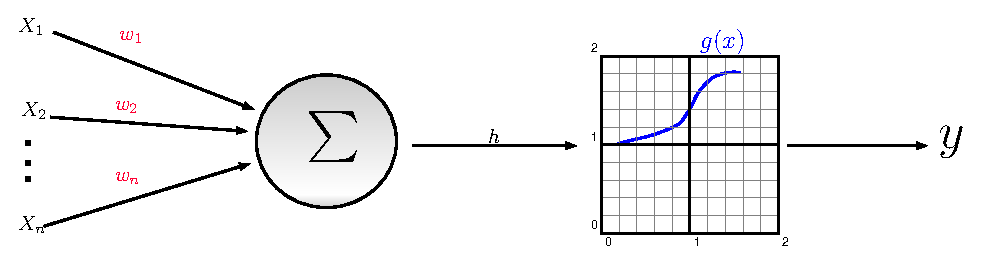
\includegraphics[scale=0.7]{Imagens/McCulloch.eps}
	}
	\caption{Modelo esquemático de um neurônio de McCulloch-Pitts. Onde $x_{1}, x_{2}, ..., x_{n}$ são os \textit{inputs}, $w_{1}, w_{2}, ..., w_{n}$ são os pesos, h é o treino, $g(x)$ é a função de ativação, e $y$ é o \textit{output}.}
	\label{Esquematico de McCulloch}
\end{figure}

Mais de $50$ tipos de redes neuronais artificiais tem sido criadas até o ano de $2014$ \citep{Saljooghi2014}.


\section{A Rede de Kohonen}

Neste trabalho, foi utilizada a rede de kohonen. Esta rede neuronal tem como importante característica ser uma rede com aprendizado não-supervisionado, portanto o espaço solução de saída da rede não é conhecido. 

A localização espacial de um neurônio da saída em um mapa topológico
corresponde a um domínio ou característica particular do dado retirado do espaço de entrada. E estas entradas são mapeadas de forma ordenada, a exemplo dos mapas cito-arqueturais do córtex cerebral.

Neste processo de identificação de padrões a redundância torna-se impreterível,
pois o neurônio da camada de saída que apresentar a maior resposta terá os seus
pesos ajustados. Além disso, o peso dos neurônios vizinhos também serão
ajustados em menor intensidade ao comparados com o neurônio vencedor.

Isto implica que os neurônios devem estar posicionados em um arranjo geométrico
adequado. Esta teoria é baseada na suposição de que as células nervosas
corticais estão organizadas anatomicamente em relação aos estímulos que recebem
dos sensores aos quais estão ligadas \citep{Artero2009}.

Este modelo exige a definição de vizinhança entre neurônios de forma geométrica. Alguns arranjos são comumente utilizados, como por exemplo, os arranjos triangulares, hexagonal, retangulares, etc.

No caso de arranjos retangulares, diferentes vizinhanças de um neurônio
$N_{i,j}$ podem ser configuradas em quartetos, diagonais e octetos. 

A Fig. \ref{hiperplano} ilustra o arranjo retangular e as vizinhanças, em quartetos, adotado neste trabalho. 

\begin{figure}[H]
	\centering
	\setlength{\fboxsep}{8pt}
	\setlength{\fboxrule}{0.1pt}
	\fbox{
		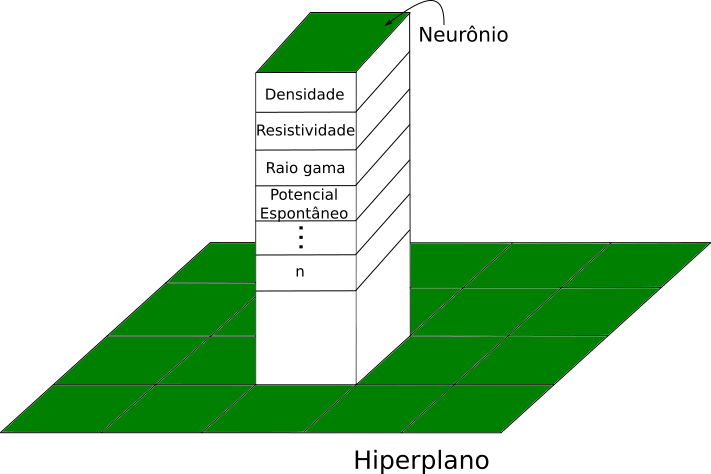
\includegraphics[scale=0.5]{Imagens/hiperplano.png}
	}
	\caption{Neurônio e suas vizinhanças}
	\label{hiperplano}
\end{figure}

O conceito de vizinhança representa uma competição pelo melhor aprendizado e o ajuste do vencedor e da sua vizinhança é um estímulo para que os neurônios ao redor do vencedor também melhorem.

Durante a etapa de treinamento é identificado o neurônio que tem os parâmetros de entrada mais parecidos com os valores dos pesos. Este procedimento é realizado via cálculo da distância euclidiana, Eq. \ref{euclidiana}, entre o parâmetro de entrada $x(t)$ e o peso $w_{i,j}$.

\begin{eqnarray}
d(t)= \sum^{n}_{i=1}[x(t)-w_{i,j}(t)]^{2}
\label{euclidiana}
\end{eqnarray}

A etapa de treinamento da rede se dá por um ajuste de pesos entre os neurônios através do cálculo do menor valor de $d(t)$ na iteração $t$, caracterizando assim o neurônio que passar por esse processo de \textit{vencedor}. Esse procedimento ajusta da mesma forma os pesos do neurônio da vizinhança dentro. Os pesos são ajustados co uma fração da diferença entre os \textit{inputs} $x_{i}$ e os pesos $w_{i}$, vide Eq.\ref{ajuste de pesos}.

\begin{equation}
w_{i,j}(t+1)=w_{i,j}(t)+n(t)[x(t)-w_{i,j}]
\label{ajuste de pesos}
\end{equation}

Através deste ajuste continuado de pesos os elementos do conjunto de entrada são reorganizados de tal foma que as classes próximas sejam posicionados umas perto das outras. Isso gera um mapa bi-dimensional denominado na literatura de \textit{mapa auto-organizável}. Este mapa é o análogo matemático mais fiel das áreas especializadas do córtex cerebral que são ilustradas pelo \textit{Homúnculo de Penfield}, \ref{homunculo}.

\section{Redes com aprendizado não-supervisionado}

Nesta categoria de RNA's são apenas inseridos os valores de \textit{input} da rede. Os \textit{output} são definidos pela própria rede que passa por um processo de treinamento não supervionado. As redes que são submetidas a este tipo de treinamento são mais indicadas para tarefas aonde são exigidos agrupamento de dados (\textit{clustering}). Neste processo uma classe deve ser atribuída aos registros da rede observando-se apenas o comportamento de seus atributos, no caso em particular deste trabalho tratam-se de propriedades geofísicas.

Uma rede com treinamento não supervisionado inspira-se no funcionamento do córtex cerebral. Neste modelo biológico, o organismo aprende a realizar alguma tarefa, por meio da identificação de padrões. Por exemplo, ao identificar uma música determinados padrões sonoros que compõe o conjunto harmonioso de notas precisam ser aprendidos antes de serem reconhecidos. Durante este processo, regiões específicas do cérebro vão sendo paulatinamente acionadas. Isto somente é possível, devido conexões específicas que são formadas entre os neurônios
presentes no córtex, Fig. \ref{homunculo}.

Os detalhes dos processos que regulam o córtex ainda não foram totalmente elucidados, contudo é seguro assumir que a primeira representação dos fenômenos de aprendizagem podem ser representados por uma superfície topológica ou mapa auto-organizado. 

\begin{figure}[H]
	\centering
	\setlength{\fboxsep}{8pt}
	\setlength{\fboxrule}{0.1pt}
	\fbox{
		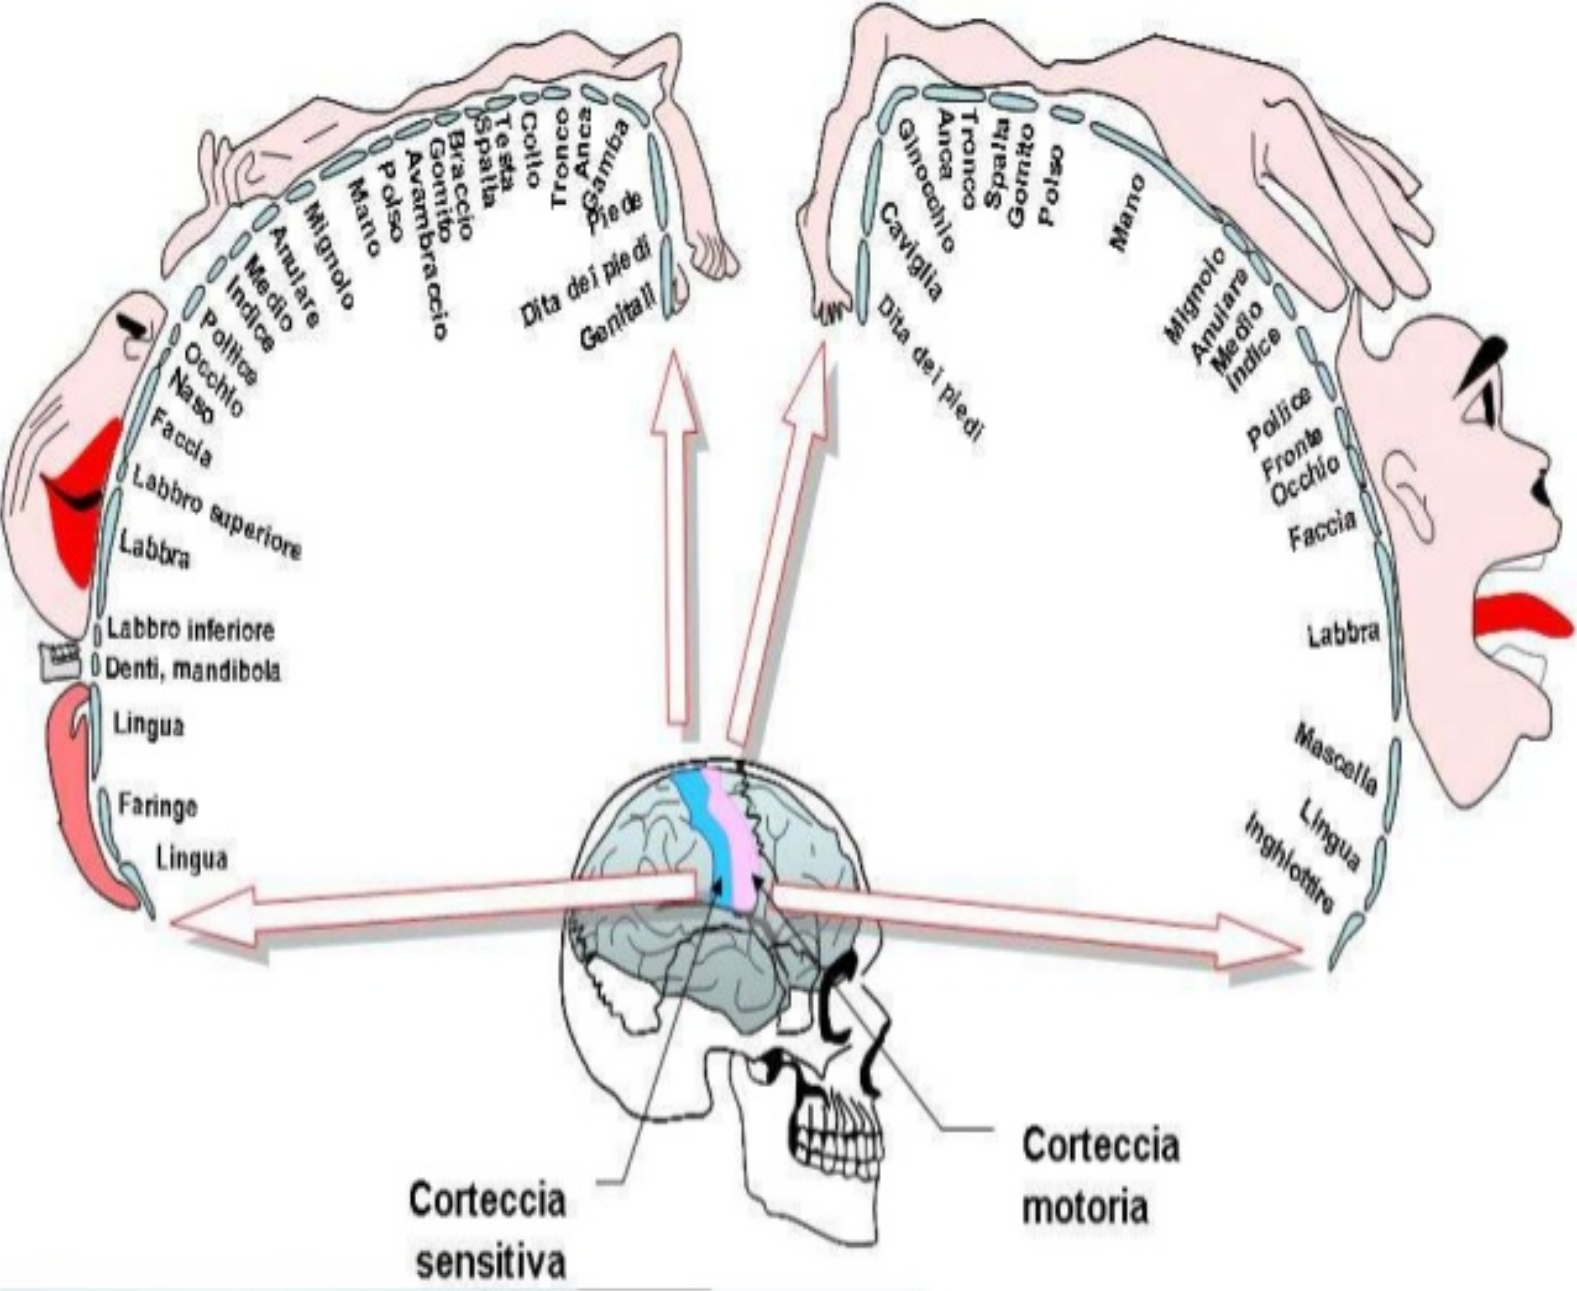
\includegraphics[scale=0.5]{Imagens/homunculo.png}
	}
	\caption{Homúnculo de Penfield.}
	\label{homunculo}
\end{figure}

Um cérebro que sofreu uma comoção grave perde a capacidade de acessar determinadas zonas do homúnculo responsáveis por atividades específicas. Contudo o cérebro tem a capacidade de destinar outras regiões para o controle destas ações que foram previamente perdidas.

Além de casos graves como um acidente o cérebro também perde a capacidade de aprendizado com o tempo. Em humanos, a capacidade de aprendizado vai da pequena infância até a puberdade. Após este período, o cérebro passar a reter o que fora aprendido. Sendo assim o aprendizado é uma função que depende, entre outras coisas, do tempo.

\section{Medidas de Semelhança}

Dado um conjunto de dados numéricos, a \textbf{métrica do dado} é qualquer leitura em uma dada escala de intervalo que infere o grau de diferença entre dois objetos.  Dados que são caracterizados como dados \textbf{não-métricos}, são aqueles conjuntos de dados que podem ser coletados em um formato \textit{binário} (0/1),  \textit{ordinário} números que expressam uma posição somente (índice), ou \textit{escala nominal} que são conjuntos de dados não ordenados \citep{Michel2016}.

Na análise geométrica do dado se refere aos aspectos geométricos da imagem, análise de padrões ou forma, que trata um conjunto arbitrário de dados como uma nuvem de pontos no espaço  $\Re ^{n}$. O dado passa a ser organizado em uma base de dados indexadas em um espaço métrico\footnote{Este processo é conhecido como indexação métrica.}.

Na análise de agrupamentos (classificação, taxonomia, reconhecimento de padrões) consiste em dividir o dado $A$ em um conjunto menor de grupos. Por exemplo, um grupo de dados que estão próximos em respeito a um determinado critério como propriedades físicas em rochas. 

Neste trabalho são estudadas duas medidas de semelhança especiais. A primeira delas e a métrica de \textit{Euclides} que leva em consideração o cálculo de centroides para avaliar a distância entre dois agrupamentos. A segunda é a métrica de \textit{Mahalanobis} que leva em consideração a forma do agrupamento a ser analisado.   

\subsection{A métrica Euclideana}

Dado dois conjuntos de agrupamentos distintos, $\theta$($\bar{x}_{i},\bar{y}_{i}$) e $\beta$($\bar{x}_{j},\bar{y}_{j}$), os seus vetores de coordenadas cartesianas podem ser definidos como

\begin{multicols}{2}
	\begin{equation}
	 \textbf{x}^{i}=
		\begin{bmatrix} 
		x_{1}^{i} \\
		x_{2}^{i} \\
		x_{2}^{i} \\
		\vdots \\
		x_{m}^{i}
		\end{bmatrix}
	\end{equation}
	
   \begin{equation}
      \textbf{y}^{i}=
    	\begin{bmatrix} 
       	y_{1}^{i} \\
    	y_{2}^{i} \\
    	y_{2}^{i} \\
	     \vdots \\
	    y_{m}^{i}
    	\end{bmatrix}
   \end{equation}
\end{multicols}

para um agrupamento $\theta$, e 

\begin{multicols}{2}

\begin{equation}
     \textbf{x}^{j}=
		\begin{bmatrix} 
		x_{1}^{j} \\
		x_{2}^{j} \\
		x_{2}^{j} \\
		\vdots \\
		x_{n}^{j}
		\end{bmatrix}
\end{equation}

\begin{equation}
      \textbf{y}^{j}=
		\begin{bmatrix} 
		y_{1}^{j} \\
		y_{2}^{j} \\
		y_{2}^{j} \\
		\vdots \\
		y_{n}^{j}
		\end{bmatrix}
\end{equation}
\end{multicols}

para outro agrupamento  $\beta$.  A métrica euclideana, na sua forma mais genérica, pode ser definida como uma distância ponderada, de acordo com a Eq. \ref{eucli}.

\begin{equation}
[(\bar{\textbf{x}_{i}}-\bar{\textbf{x}}_{j})^{T}\textbf{A}(\bar{\textbf{y}}_{i}-\bar{\textbf{y}}_{j})]^{1/2}
\label{eucli}
\end{equation}

Onde $\textbf{A}$ é uma matriz não-singular e simétrica de dimensão $m \times n $ e com $m=n$, $\bar{\textbf{x}}_{i}$ é a média do vetor de coordenadas cartesianas do agrupamento $\theta$ com dimensão $m$, $\bar{\text{y}}_{i}$ é a média do segundo vetor de coordenadas do agrupamento $\theta$ com dimensão $m$, $\bar{\textbf{x}}_{j}$ é a média do vetor de coordenadas do agrupamento $\beta$ com dimensão $n$, $\bar{\textbf{y}}_{j}$ é a média do segundo vetor de coordenadas cartesianas do agrupamento $\beta$ também com dimensão $n$.

Nos casos em que $\textbf{A} = \textbf{I}$, onde $\textbf{I}$ é a matriz identidade obtém-se a métrica euclideana não-ponderada, que é o caso estudado neste trabalho. 

A métrica euclideana é de fácil compreensão. Contudo sua utilização apenas apresenta bons resultados, quando todas as classes possuam a mesma variância. Além disso, os elementos dos vetores não devem possuir nenhum tipo de correlação entre si, em resumo, estes devem ser circulares. E no espaço de propriedades, onde os elementos dos vetores se distribuem, isso raramente ocorre. 

\subsection{A métrica de Mahalanobis}

A distância de Mahalanobis é um caso particular da métrica euclideana onde, no lugar da matriz $\textbf{A}$, utiliza-se a matriz de covariância agrupada inversa $\textbf{S}$. Esta métrica mede a separação entre dois grupos de objetos levando-se em consideração o formato da distribuição dos dados. Suponhamos que nós tenhamos dois grupos de objetos com médias $\bar{\textbf{x}}_{i}$ e $\bar{\textbf{x}}_{j}$, a distância de Mahalanobis é dado pelo seguinte enunciado, Eq. \ref{maha}:

\begin{equation}
[(\bar{\textbf{x}_{i}}-\bar{\textbf{x}}_{j})^{T}\textbf{S}^{-1}(\bar{\textbf{y}}_{i}-\bar{\textbf{y}}_{j})]^{1/2}
\label{maha}
\end{equation}

Os dados dos dois grupos devem ter o mesmo número de variáveis (o mesmo número de colunas), mas não necessariamente o mesmo número de dados (cada grupo pode possuir diferentes número de linhas). A matriz covariância para o grupo $i$ é calculada usando uma matriz de dados centralizada $\hat{\textbf{X}}$.


\begin{equation}
\textbf{C}_{i}=\dfrac{1}{n} \hat{\textbf{X}_{i}}^{T}\hat{\textbf{X}_{i}}
\end{equation}

Onde $n=\sum_{i} n_{i}$, ou seja a soma de todos os dados de todos os grupos. 


A matriz de covariância agrupada $\textbf{S}$ (\textit{Pooled Covariance Matrix}) dos dois agrupamentos ($\theta, \beta$) é computada como a média ponderada das matrizes de covariância:

\begin{equation}
\textbf{S}(\theta, \beta)=\dfrac{1}{n}\sum^{g}_{i=1}n_{i}C_{i}
\end{equation}

Onde $\theta$ e $\beta$ representam os dois agrupamentos e $g$ é o número de agrupamentos.


\subsection{Análise de agrupamento}
\label{teste}

Ao se criar uma análise de agrupamentos tem-se em vista a caracterização do quão semelhante, ou não, dois ou mais conjuntos de dados podem ser.  Para se determinar em qual situação cada métrica se comporta melhor, foi gerado um teste analítico com vistas a se comparar tanto a distância quanto a forma da distribuição dos dados influem no valor absoluto final das duas métricas. 

No primeiro teste, gerou-se distribuições randômicas circulares de três agrupamentos com seus centros igualmente espaçados como apresentado na Fig. \ref{AC1}. Nota-se que os clusters encontram-se a $20$ unidades de distância entre seus respectivos centros. 

\begin{figure}[H]
	\centering
	\setlength{\fboxsep}{8pt}
	\setlength{\fboxrule}{0.1pt}
	\fbox{
		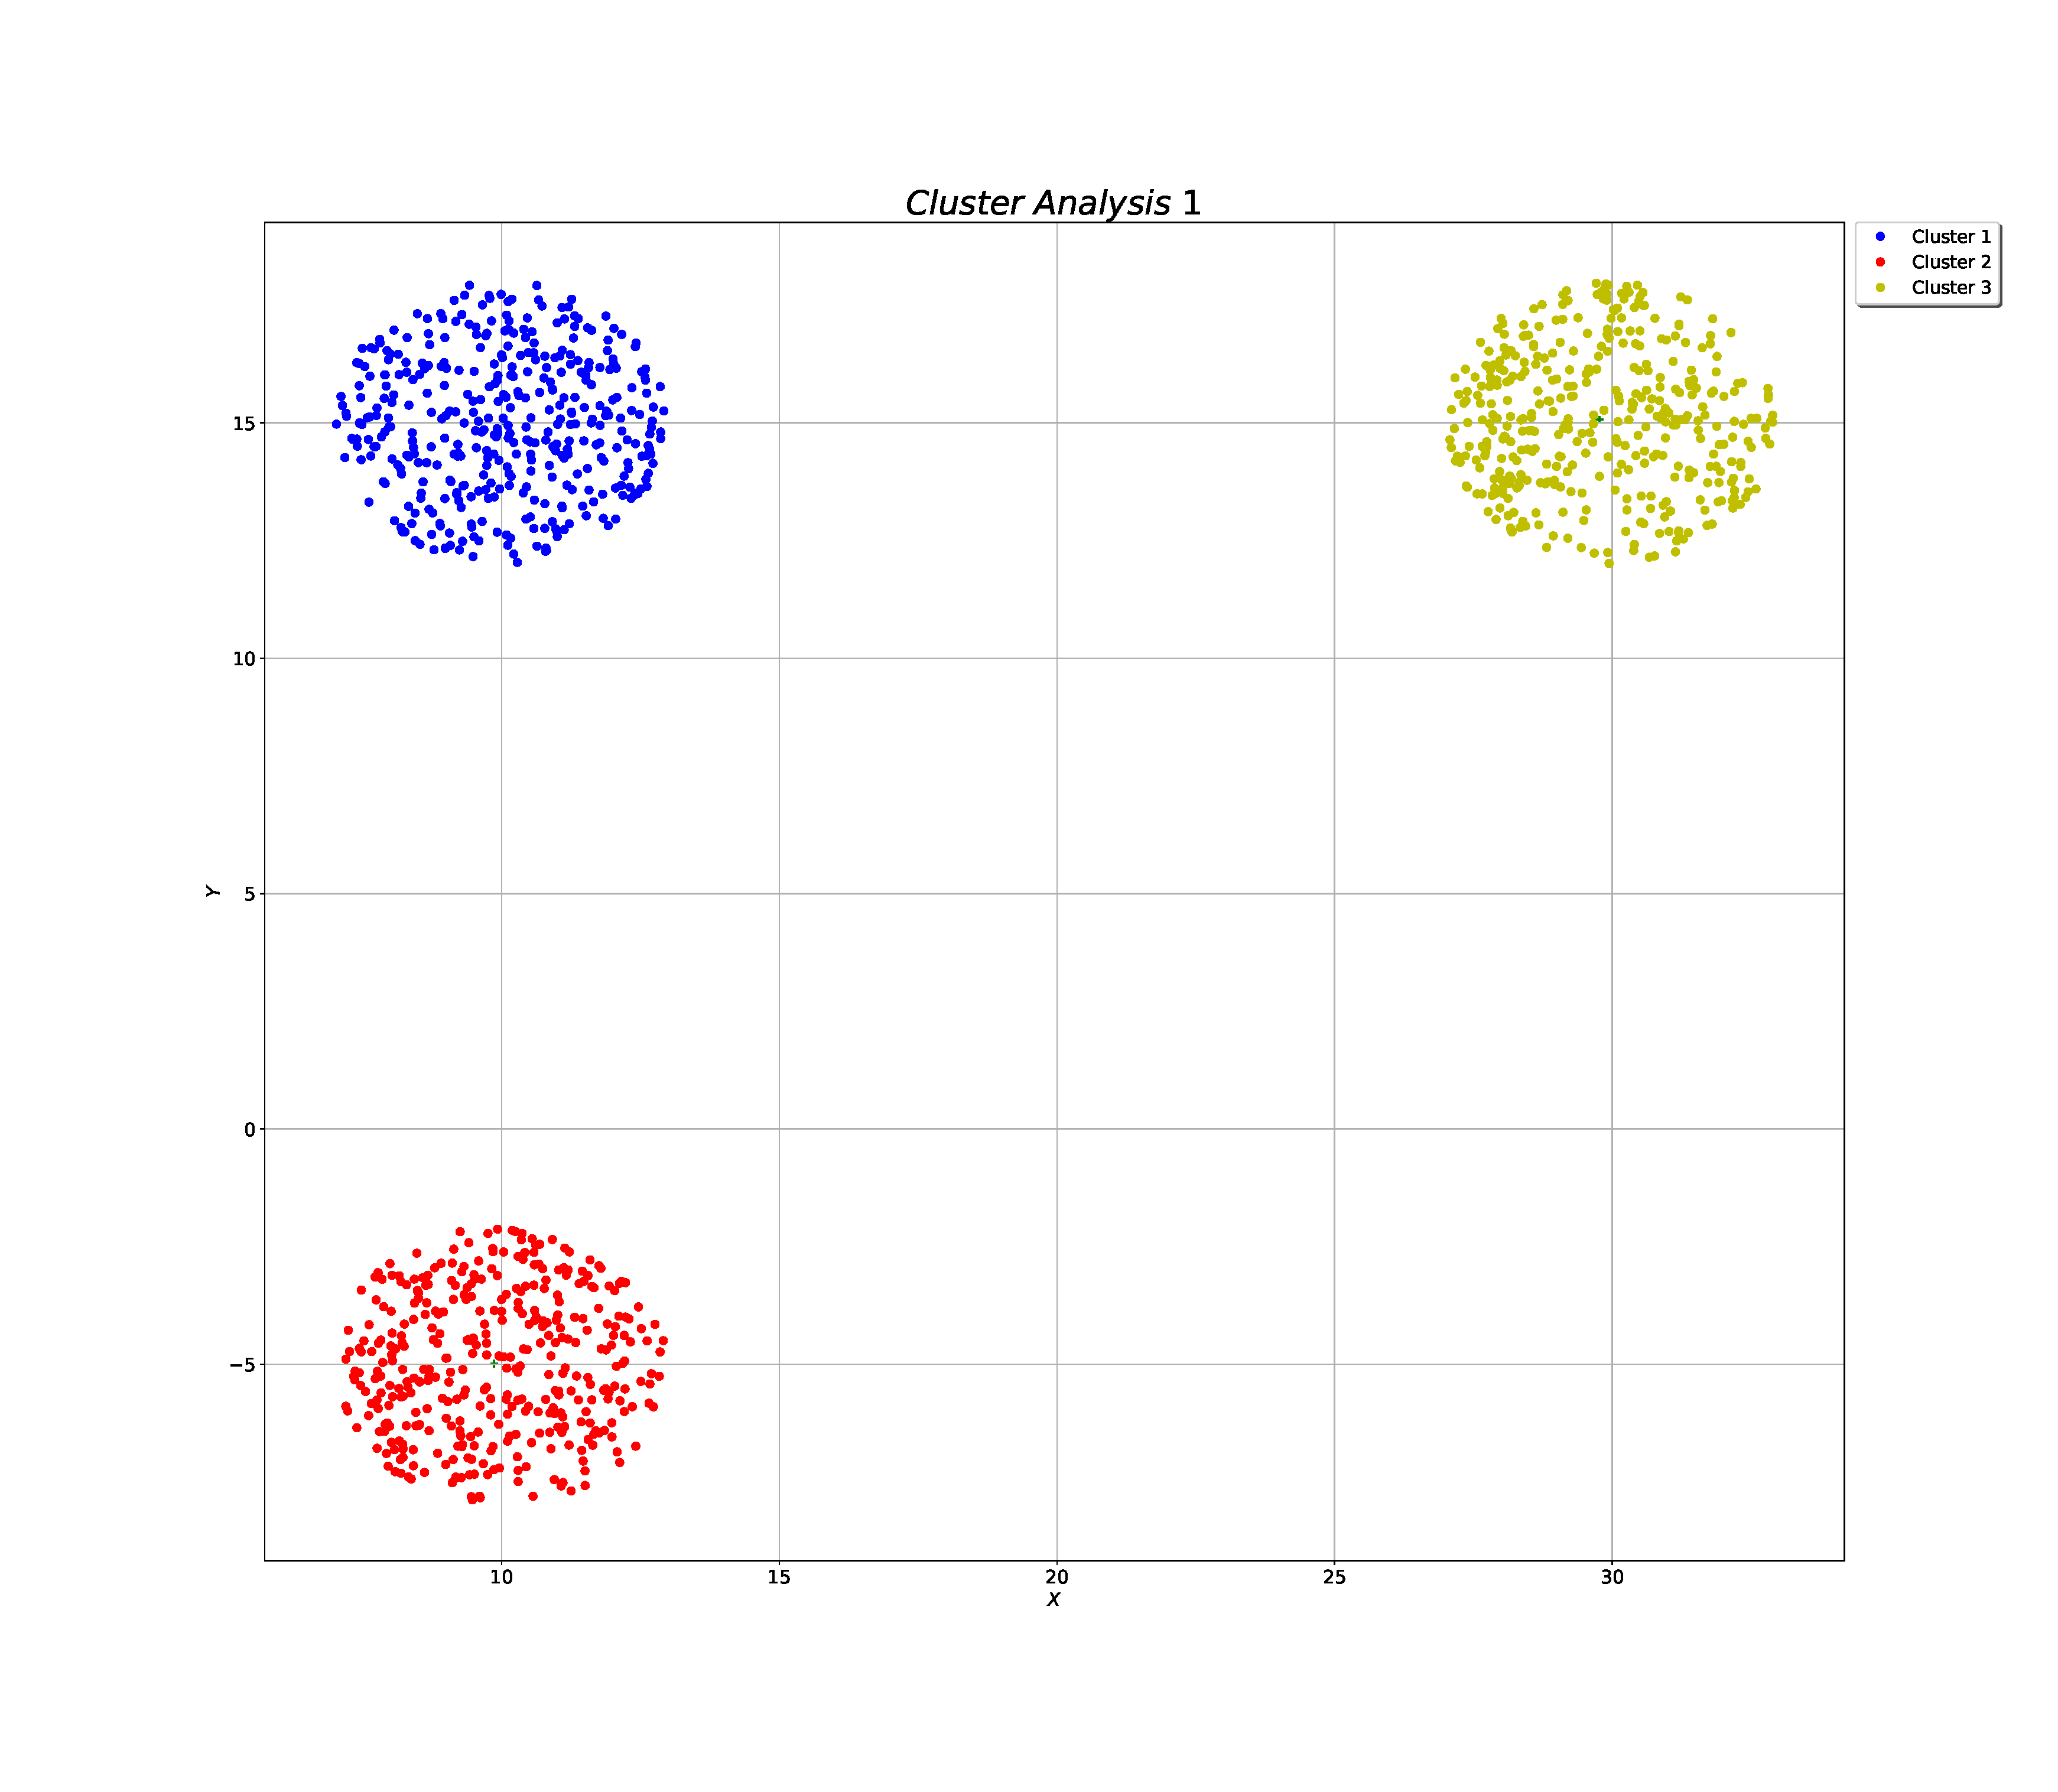
\includegraphics[scale=0.20]{Imagens/clusteranalise1.eps}
	}
	\caption{Análise de agrupamento 1}
	\label{AC1}
\end{figure}

O primeiro caso estudado apresentam três circunferências compostas por diferentes conjuntos de dados. Os parâmetros utilizados para criar a primeira situação de estudo são apresentadas na Tab. \ref{analise1}.

\begin{table}[H]
	\centering
	\caption{Parâmetros dos teste analítico para comparação das métricas.}
	\label{analise1}
	\begin{tabular}{lccc}
		\hline
		Parâmetros       & \textcolor{blue}{Cluster1} & \textcolor{red}{Cluster 2} & \textcolor{olive}{Cluster 3} \\ \hline
		Raio máximo      & 0.300E+01 & 0.300E+01 & 0.300E+01 \\
		Raio mínimo      & 0.000E+00 & 0.000E+00 & 0.000E+00 \\
		Ângulo máximo    & 0.157E+02 & 0.157E+02 & 0.157E+02 \\
		Ângulo mínimo    & 0.000E+00 & 0.000E+00 & 0.000E+00 \\
		Semente                & 5                 & 5                  & 5         \\
		Número de pontos & 404       & 383       & 397   \\        \hline
	\end{tabular}
\end{table}

Para os casos em que a distribuição, no espaço de propriedades, apresenta simetria em ambos os eixos as métricas apresentam uma pequena diferença entre si. A distância de Euclides medida entre os agrumamentos I e II foi de $20,0$ unidades de medida, enquanto que a mesma distância medida entre os clusters I-III foi de $19,8$ unidades de medida. Tal diferença se deve a imprecisão associada ao sorteio randômico e o deslocamento dos centros das distribuições. 

A distância de Mahalanobis leva em consideração a forma das distribuições de dados ao longo do espaço de propriedades.  O resultado desta métrica para os agrupamentos I-II foi de $13,8$, enquanto que a mesma métrica para os agrupamentos I-III foi de $12,9$. Mostrando que os resultados se afastam um pouco mais.
 
 \begin{table}[H]
 	\centering
 	\label{metrica1}
 	\begin{tabular}{|l|l|}
 		\hline
 		\multicolumn{2}{|c|}{Distâncias}  \\ \hline
 		Euclideana (I-II)     & 0.200E+02 \\ \hline
 		Mahalanobeana (I-II)  & 0.138E+02 \\ \hline
 		Euclideana (I-III)    & 0.197E+02 \\ \hline
 		Mahalanobeana (I-III) & 0.129E+02 \\ \hline
 	\end{tabular}
 \end{table}


O segundo teste apresenta uma leve deformação no agrupamento I (em \textcolor{blue}{azul}), Fig. \ref{AC2}.  Um pequeno aumento do eixo horizontal muda a distribuição para uma forma levemente elipsoidal de dados no espaço. Os demais clusters continuam com uma distribuição circular.



\begin{figure}[H]
	\centering
	\setlength{\fboxsep}{8pt}
	\setlength{\fboxrule}{0.1pt}
	\fbox{
		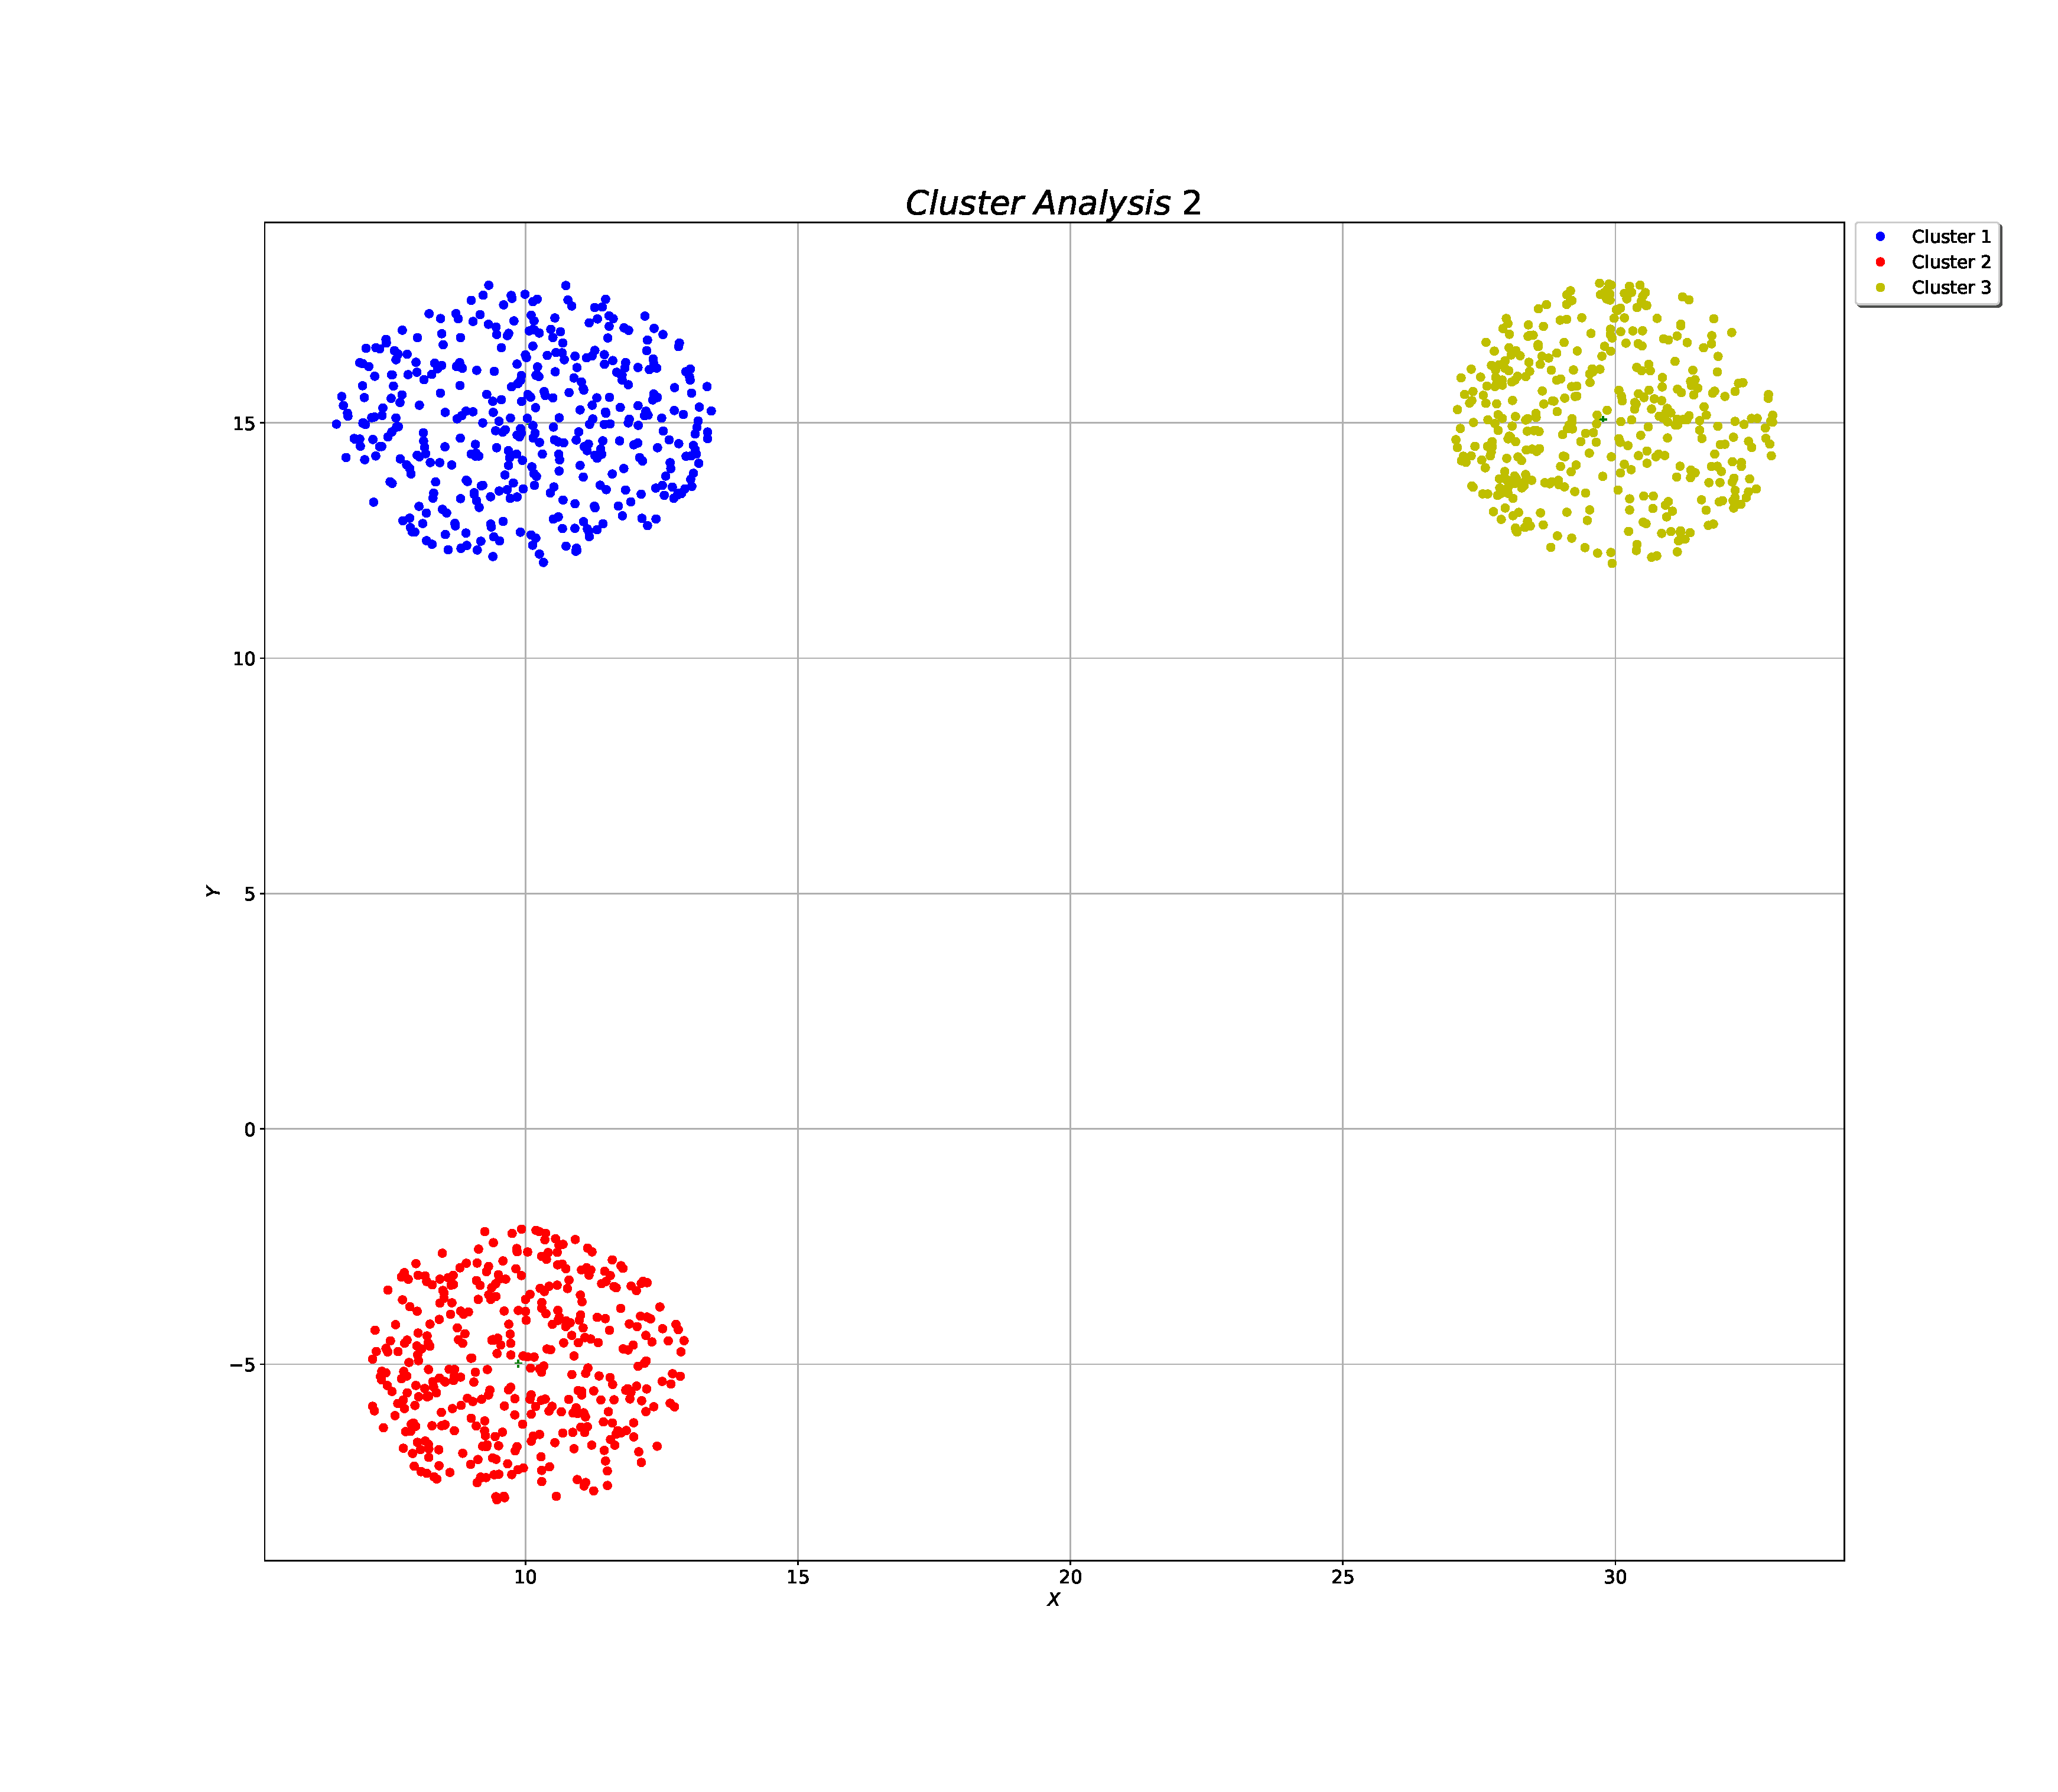
\includegraphics[scale=0.20]{Imagens/clusteranalise2.eps}
	}
	\caption{Análise de agrupamento 2}
	\label{AC2}
\end{figure}

A Tab. \ref{analise2} mostram os parâmetros utilizados para a criação de cada um dos clusters. Salienta-se a principal mudança foi um leve aumento do eixo horizontal da ordem de $0,5$ unidades de medida. Os demais parâmetros tais como posição e número de dados dos clusters permaneceram inalterados. 

\begin{table}[H]
	\centering
	\caption{Parâmetros do segundo teste analítico.}
	\label{analise2}
	\begin{tabular}{lccc}
		\hline
		Parâmetros       & \textcolor{blue}{Cluster1} & \textcolor{red}{Cluster 2} & \textcolor{olive}{Cluster 3} \\ \hline
		Raio máximo      & --- & 0.300E+01 & 0.300E+01 \\
		Raio mínimo      & --- & 0.000E+00 & 0.000E+00 \\
		Ângulo máximo    & 0.157E+02 & 0.157E+02 & 0.157E+02 \\
		Ângulo mínimo    & 0.000E+00 & 0.000E+00 & 0.000E+00 \\
		Eixo maior        & 0.350E+01        & ----         & ---         \\
		Eixo menor          & 0.300E+01        & ---       & ---        \\
		Semente          & 9         & 9         & 9         \\
		Número de pontos & 405       & 383       & 396   \\   \hline
	\end{tabular}
\end{table}

No segundo caso, a distância de Euclides permaneceu inalterada para ambos os casos, tanto na distância entre os agrupamentos I-II e I-III. Isso se deve ao fato de os centroides permanecerem inalterados para as análises de agrupamentos 1 e 2, observando-se um valor de $20,0$ e $19,7$ unidades de distância. 
A distância de Mahalanobis sofreu o maior impacto no seu valor absoluto, na ordem de $2$ unidades de medida entre os agrupamentos I-III. De maneira geral os padrões de comportamento das métricas permaneceram inalterados, com exceção do caso aonde a Mahalanobis foi de $11,8$ unidades de medida demonstrando a sensibilidade esperada para deformações em grupos de dados. Enquanto que o valor encontrado para o agrupamento I-II foi de $13,8$, muito semelhante ao do teste anterior. 

 \begin{table}[H]
 	\centering
 	\label{metrica2}
 	\begin{tabular}{|l|l|}
 		\hline
 		\multicolumn{2}{|c|}{Distâncias}  \\ \hline
 		Euclideana (I-II)     & 0.200E+02 \\ \hline
 		Mahalanobeana (I-II)  & 0.138E+02 \\ \hline
 		Euclideana (I-III)    & 0.197E+02 \\ \hline
 		Mahalanobeana (I-III) &  0.118E+02 \\ \hline
 	\end{tabular}
 \end{table}


O terceiro teste apresenta o agrupamento 1 com um formato elipsoidal oblato se aproximando mais do agrupamento 3. Este comportamento é retratado na Fig. \ref{AC3}. Os demais conjuntos de agrupamentos permaneceram com a mesma forma dos testes anteriores. 

\begin{figure}[H]
	\centering
	\setlength{\fboxsep}{8pt}
	\setlength{\fboxrule}{0.1pt}
	\fbox{
		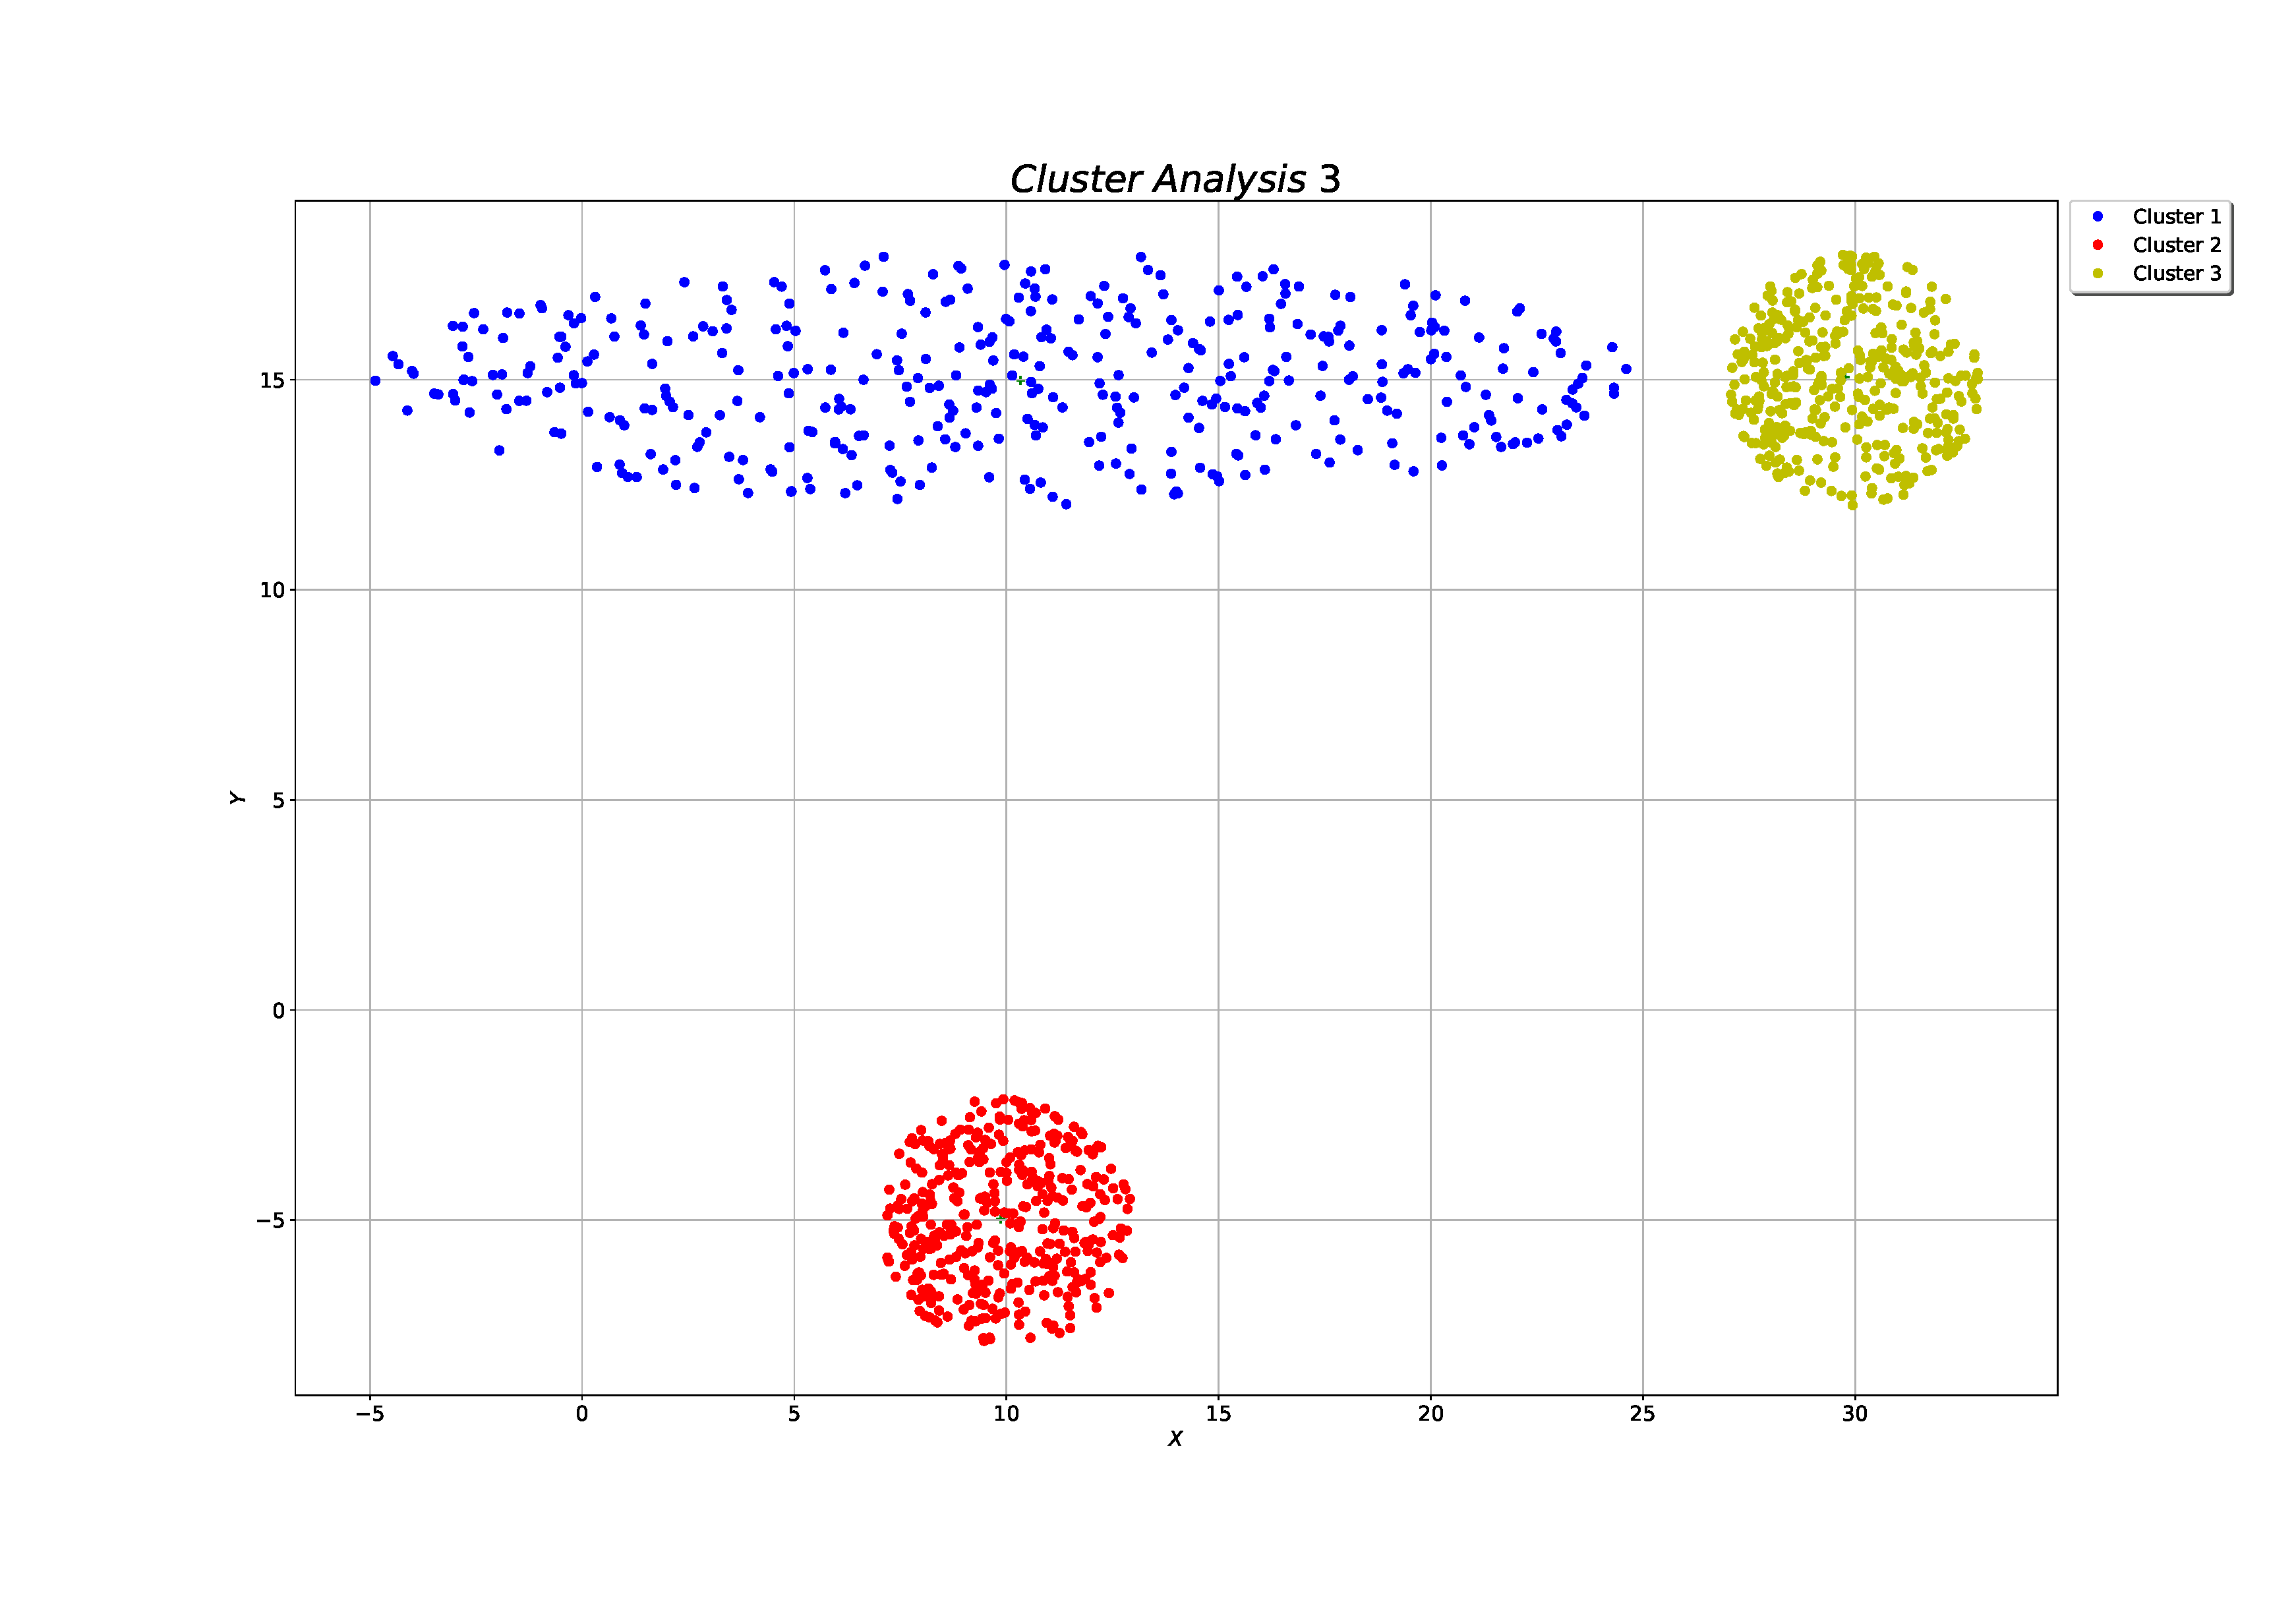
\includegraphics[scale=0.25]{Imagens/clusteranalise3.eps}
	}
	\caption{Análise de agrupamento 3}
	\label{AC3}
\end{figure}


A deformação explícita no agrupamento 1 se deu por conta do aumento de $11,5$ unidades de medida do eixo horizontal. Essa perturbação na forma da elipse em contraste com os demais clusters é descrita na Tab. \ref{analise3}.


\begin{table}[H]
	\centering
	\caption{Parâmetros dos teste analítico para comparação das métricas.}
	\label{analise3}
	\begin{tabular}{lccc}
		\hline
		Parâmetros       & \textcolor{blue}{Cluster1} & \textcolor{red}{Cluster 2} & \textcolor{olive}{Cluster 3} \\ \hline
		Raio máximo      & --- & 0.300E+01 & 0.300E+01 \\
		Raio mínimo      & --- & 0.000E+00 & 0.000E+00 \\
		Ângulo máximo    & 0.157E+02 & 0.157E+02 & 0.157E+02 \\
		Ângulo mínimo    & 0.000E+00 & 0.000E+00 & 0.000E+00 \\
		Eixo maior        & 0.150E+02        & ----         & ---         \\
		Eixo menor          &  0.300E+01        & ---       & ---        \\
		Semente          & 17         & 17         & 17         \\
		Número de pontos & 405       & 384       & 395  \\   \hline
	\end{tabular}
\end{table}


 \begin{table}[H]
 	\centering
 	\label{metrica3}
 	\begin{tabular}{|l|l|}
 		\hline
 		\multicolumn{2}{|c|}{Distâncias}  \\ \hline
 		Euclideana (I-II)     & 0.200E+02 \\ \hline
 		Mahalanobeana (I-II)  & 0.138E+02 \\ \hline
 		Euclideana (I-III)    & 0.194E+02 \\ \hline
 		Mahalanobeana (I-III) & 0.352E+01 \\ \hline
 	\end{tabular}
 \end{table}

A distância de Euclides permaneceu inalterada dos três casos estudados entre os três agrupamentos. Apresentando o valor de $2,0$ e $19,4$ para as distâncias entre os agrupamentos I-II e I-III respectivamente. Contudo, o cômputo da distância de Mahalanobis apresentou uma grande diferença se comparado as análises anteriores. Apresentando o valor de $13,8$ unidades de medida entre os agrupamentos I-II e $3,5$ unidades de medida entre os agrupamentos I-III.  

Esta pequena análise demonstra que o cômputo da distância de Mahalanobis está intimamente relacionada com a forma da distribuição dos dados dentro do espaço de propriedades quando comparada a distância Euclideana. Isto se deve ao cálculo da matriz de covariância para cada classe de dados \ref{maha}, que permite levar em conta a forma do agrupamento em questão. 



  \chapter{Contexto Geológico}
A Bacia do Paraná desenvolveu-se sobre uma área de escudo do continente Gondwana Sul e é composta por uma série de núcleos cratônicos, rodeados por vários cinturões móveis e cobertos por bacias molássicas, que foram desenvolvidas durante o ciclo termo-tectônico Brasiliano que se estendeu desde o neoproterozóico até o Ordoviciano. A deformação decorrente deste ciclo teve início entre $700$ Ma e $650$ Ma, sendo que a maior parte das intrusões de granitos que podemos observar na Bacia, situou-se dentro do limite entre o Proterozóico e o Paleozóico (cerca de $570$ Ma) com resfriamento durante o Cambro-Ordoviciano entre $500-450$ Ma \citep{zalan_p._v._tectonica_1987, hawkesworth_tectonic_2000}.

O embasamento que circunda a Bacia do Paraná é dividido em: margem Leste/Sudeste, representado pelas faixas Dom Feliciano e Ribeira ,de idade Brasiliana e de direção NE-SW, separados por um núcleo cratônico designado Rio de La Plata/ Luiz Alves; margem Norte/Nordeste, representada pela faixa Uruaçu, de idade mesoproterozóica, de direção NW e por dois maciços arqueanos (Guaxupé e Goiás) remobilizados durante o ciclo Brasiliano; margem Oeste/Noroeste representada pela faixa de dobramentos Paraguai/Araguaia, também do ciclo Brasiliano, que delimita o extremo da borda Noroeste da Bacia \citep{borghi_2002, hawkesworth_tectonic_2000}.

Dentre os principais grupos de estruturas, nota-se três grupos de lineamentos de direções preferenciais NW-SE, E-W e NE-SW, representando cada um evento termo-tectônico distinto. O conjunto de lineamentos NW-SE são os mais antigos e estão relacionados ao evento  termo-tectônico do Transamazônico, e, as zonas de falhas geológicas associadas a este evento foram reativadas durante o rifteamento do Atlântico Sul, no Cretáceo.  Os lineamentos E-W, tiveram início a partir do Triássico e são paralelos às zonas de fratura oceânica, sugerindo uma ligação com o desenvolvimento do Atlântico Sul. Os lineamentos NE-SW são derivados do evento tremo-tectônico Brasiliano e de seus cinturões móveis associados. Este último conjunto de lineamentos é isento de diques de basalto \citep{milani_outline_1999}. 

O registro estratigráfico da Bacia do Paraná é formado por pacote sedimentar e magmático de espessura máxima em torno de $7000$ m, que coincide geograficamente com o depocentro estrutural da sinéclise e com a calha do rio paraná \citep{milani_orogenias_1998}. O registro estratigráfico da Bacia do Paraná é dividido em seis unidades de ampla escala ou supersequências \citep{Vail_1977} na forma de pacotes rochosos com intervalos temporais de algumas dezenas de milhões de anos de duração e envelopados por superfícies de discordância de caráter inter-regional: Rio Ivaí (Ordoviciano-Siluriano), Paraná (Devoniano), Gondwana I (Carbonífero-Eotriássico), Gondwana II (Meso a Neotriássico), Gondwana III (Neojurássico-Eocretáceo) e Bauru (Neocretáceo). As três primeiras supersequências são representadas por sucessões sedimentares que definem ciclos transgressivos e regressivos ligados às oscilações do nível relativo do mar, durante o Paleozóico, ao passo que as demais correspondem a pacotes de sedimentos continentais com rochas ígneas associadas. As unidades formais da litoestratigrafia, quais sejam os grupos, formações e membros comumente utilizados na descrição do arranjo espacial dos estratos da bacia, inserem-se como elementos particularizados neste arcabouço aloestratigráfico de escala regional \citep{boletim_2007}.

O mapa geológico (Fig. \ref{mapa geologico}) apresenta a extensão e os limites da Bacia do Paraná \citep{Vidotti_2003}.



\begin{figure}[H]
	\centering
	\setlength{\fboxsep}{8pt}
	\setlength{\fboxrule}{0.1pt}
	\fbox{
		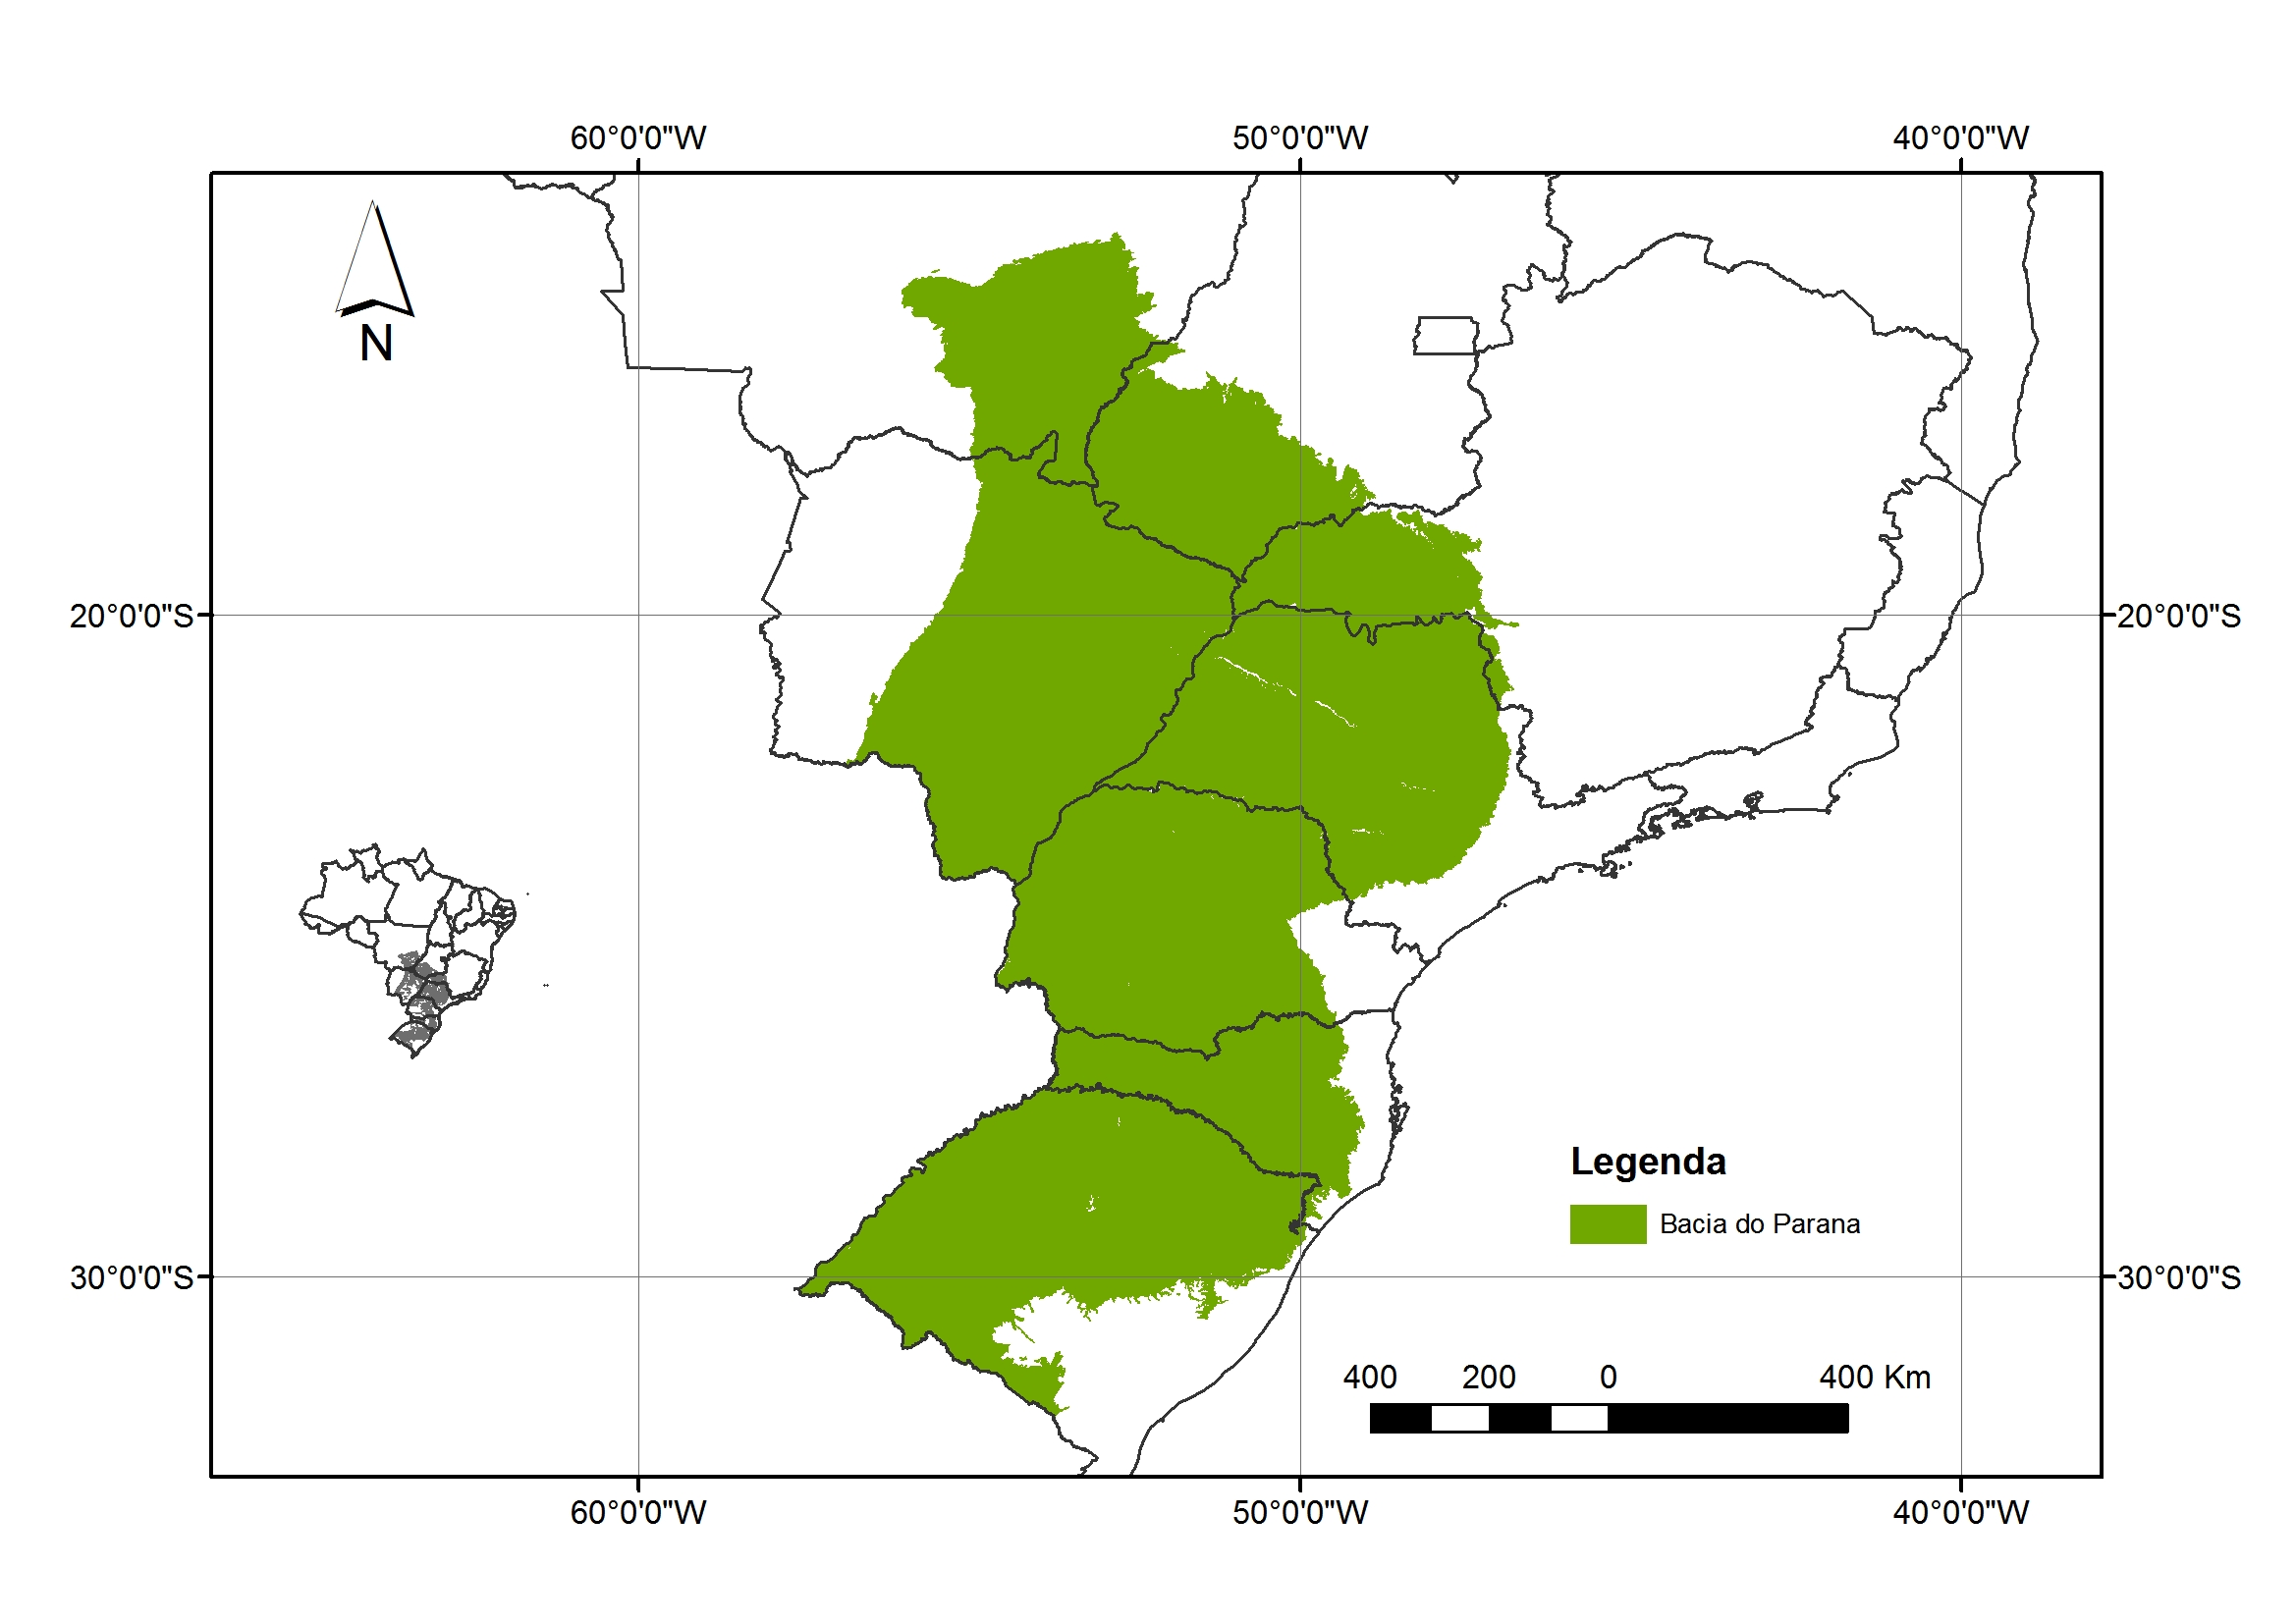
\includegraphics[scale=0.4]{Imagens/BaciaParana.jpg}
	}
	\caption{Mapa geológico e de localização da área de estudo. }
	\label{mapa geologico}
\end{figure}


  \chapter{Método Proposto e Objetivo}

A parte operacional da metodologia divide-se em três etapas: 1- Geração de dados sintéticos, 2- Treinamento e 3- Identificação. Cada uma destas etapas será realizada por um programa computacional específico, estes programas vão funcionar de forma independente.

O primeiro programa tem por objetivo gerar dados sintéticos que devem simular os resultados obtidos num levantamento de um perfil composto.
\usetikzlibrary{calc,trees,positioning,arrows,chains,shapes.geometric,%
	decorations.pathreplacing,decorations.pathmorphing,shapes,%
	matrix,shapes.symbols}
\tikzset{
	>=stealth',
	punktchain/.style={
		rectangle, 
		rounded corners, 
		% fill=black!10,
		draw=black, very thick,
		text width=10em, 
		minimum height=3em, 
		text centered, 
		on chain},
	line/.style={draw, thick, <-},
	element/.style={
		tape,
		top color=white,
		bottom color=blue!50!black!60!,
		minimum width=8em,
		draw=blue!40!black!90, very thick,
		text width=10em, 
		minimum height=3.5em, 
		text centered, 
		on chain},
	every join/.style={->, thick,shorten >=1pt},
	decoration={brace},
	tuborg/.style={decorate},
	tubnode/.style={midway, right=2pt},
}

\begin{figure}[H]
\centering
\begin{tikzpicture}
[node distance=.8cm,
start chain=going below,]
\node[punktchain, join]  {Modelo de Bacia};
\node[punktchain, join]   {Dados da Literatura};
\node[punktchain, join]   {Estimar erros das propriedades físicas para dada litologia};
\node[punktchain, join] {Definir taxa de amostragem};
\node[punktchain, join, ] {Gerar dados sintéticos contaminados com o erro gaussiano estimado};

\end{tikzpicture}
\caption{Fluxograma do programa de geração dos dados sintéticos}
\end{figure}


O programa da etapa de Treinamento será alimentado com dados de perfilagens cujas respectivas fácies litológicas são conhecidas (inicialmente serão usados dados sintéticos e posteriormente dados reais). Este programa vai gerar um arquivo com os dados do treinamento, que será usado pelo programa de Operação. Esta é a fase de aprendizagem da rede.


\begin{figure}[H]
	\centering
	\begin{tikzpicture}
	[node distance=.8cm,
	start chain=going below,]
	\node[punktchain, join]  {Início};
	\node[punktchain, join] (L1)  {Entrar com os dados do treinamento};
	\node[punktchain, join]   {Atualizar o peso do neurônio vencedor};
	\node[punktchain, join] (L2) {Fazer alteração nas vizinhanças do neurônio vencedor. Varre os dados de forma sequencial};
	\node[punktchain, join, ] {Avaliar o nível de treinamento da rede};
	\node[punktchain, join, ] {\color{red}Caso não esteja satisfatório volta-se para o Início e repete o processo de forma acumulativa};
	\node[punktchain, join, ] {\color{blue}Caso esteja satisfatório é o decretado o final do treinamento};	
	\end{tikzpicture}
	\caption{Fluxograma do programa de treinamento da rede neuronal de kohonen.}
\end{figure}

O programa da etapa de identificação vai fazer a classificação, de forma autônoma, das facies litológicas em poços a partir dos dados de perfilagem em poços nos quais a litologia é desconhecida. A aprendizagem da rede deve ocorrer de forma continuada, quanto mais informação temos sobre situações nas quais a litologia é conhecida mais bem preparada estará a rede em termos de aprendizagem. Este conceito de aprendizagem é acumulativo e isso ocorrerá através da atualização do arquivo com os dados de treinamento.

\begin{figure}[H]
	\centering
	\begin{tikzpicture}
	[node distance=.8cm,
	start chain=going below,]
	\node[punktchain, join]  {Entrada do dado não classificado};
	\node[punktchain, join] (L1)  {Determinação da distância entre os dados de cada neurônio };
	\node[punktchain, join]   {Armazena as distâncias};
	\node[punktchain, join] (L2) {Seleciona a menor distância};
	\node[punktchain, join, ] {Classifica o dado};	
	\end{tikzpicture}
	\caption{Fluxograma do programa de identificação da rede.}
\end{figure}

Durante a elaboração dos programas será necessário testar a usa eficiência. Estes testes serão realizados através de dados sintéticos que serão gerados por um terceiro programa, gerador de dados sintéticos. Este programa será alimentados com informações da literatura. Após os testes com dados sintéticos a metodologia será validada com dados reais, posteriormente depois de cumpridas todas estas etapas, a metodologia estará pronta para ser utilizada em situações reais.

É importante salientar que neste método o conhecimento do funcional geofísico, que rege a relação entre litologia e as propriedades físicas das rochas, não é necessário durante o processo. O conceito de inteligência artificial que será utilizado prescinde do funcional geofísico, o aprendizado é feito através da identificação de padrões recorrentes, sendo este ponto positivo na metodologia, pois o funcional geofísico, que por vezes é desconhecido ou de alta complexidade, exige uma modelagem matemática custosa.

O ponto negativo é a necessidade de se ter muitos dados já analisados em situações conhecidas e variadas para a realização da etapa de treinamento. A etapa de treinamento tem um custo computacional alto.

%\begin{center}
%\smartdiagram[flow diagram:vertical]{Modelo, Dados da literatura, Erro, Taxa de amostragem, Dado sintéticos}
%\end{center}



\section{Objetivo}
O principal objetivo deste projeto é desenvolver um programa computacional do tipo “ machine learning ”, que será implementado na forma de uma Rede Neuronal Artificial (RNA) dentro do contexto da inteligência artificial. Este programa deve ter a capacidade de identificar, de forma autônoma, fácies litológicas a partir de dados de perfilagem de poços sem a necessidade do uso de um funcional geofísico.

É importante salientar que a metodologia que será desenvolvida neste projeto tem aplicação direta tanto na indústria de exploração mineral, quanto na de água, e na de petróleo e gás.

  \chapter{Dados de Perfilagem}

As RNAs são capazes de reconhecer padrões \citep{Konate2014,Kumar2015}. E padrões muitas vezes são recorrentes no tocante a geologia \citep{Vail_1977}. 

Ciclos de deposição de siltes e argilas e areias muitas vezes são controlados pelas variações constantes das estações do ano \citep{Milani1998,CristinaLopesQuintas1999,Milani2000} . Esse registro litológico se faz presente em dados de poços em todo o mundo \citep{Scherer2006}.

Em uma perfilagem de poço composta são realizadas diversas medidas de propriedades físicas que ao serem analisadas, em conjunto, tornam possível ao geólogo identificar mudanças litológicas e consequentemente topos e bases de camadas de interesse \citep{FrancaAlmerio&Potter1991,Zalan2007,artur_paleoestruturas_2008}. 

A Fig. \ref{PerfilComposto} ilustra a disposição de um perfil de poço associado com topos e bases de rochas. 

\begin{figure}[H]
		\centering
	\setlength{\fboxsep}{8pt}
	\setlength{\fboxrule}{0.1pt}
	\fbox{
	\includegraphics[scale=0.16]{Imagens/poco.png}
}
	\caption{Exemplo de um dado público de uma perfilagem de poço composta realizada pela Petrobras, na Bacia do Paraná.}
	\label{PerfilComposto}
\end{figure}

Entretanto não é toda a perfilagem de poço que contém o topo e base de camada. As RNAs se apresentam como uma solução para o problema de identificação litológica e dos topos e bases dessas camadas. Uma vez observado que a variação das propriedades físicas das rochas em subsuperfície variam obedecendo certos padrões \citep{Yan2014}. 

Em \citet{Telford_1993}, encontram-se variações das propriedades físicas dos principais grupos de rochas. A Tab. \ref{rock-properties1} e a Tab. \ref{rock-properties2} apresentam um compêndio desses principais valores.  

\begin{table}[H]
	\centering
	\caption{Compilação de Perfis usados na inferência de litologia.}
	\label{rock-properties1}
	\begin{tabular}{@{}llllllllll@{}}
		\toprule
		Rocha         & Densidade ($g/cm^{3}$) & Raios-Gama ($Ci/g$)& Potencial-Espontâneo ($mV$)&   \\ \midrule
		Conglomerado &     $2,50$  &       ---        &    ---        &      \\
		Arenito  &    $2,35$      &       $2,00\leftrightarrow4,00$       &     ---       &      \\
		Folhelho &   $2,40$       &      ---        &      ---      &    \\
		Argilito &     $2,55$   &          ---     &       ---     &     \\
		Siltito  &      $2,21$    &          ---     &       ---     &   \\
		Dolomita &     $2,70$    &        $8,00$       &   ---         &       \\
		Marga  &    $2,50$     &         ---      &    ---        &     \\
		Basalto  &     $2,99$    &          $0,50$     &    ---       &      \\
		Diabásio &    $2,90$    &         ---      &       ---     &     \\
		Lava &     $2,61$    &      $0,33$         &      ---      &      \\
		Granito &    $2,64$      &       $0,70\leftrightarrow4,80$        &      ---      &      \\
		Gabro &    $3,03$     &       ---        &     ---       &       \\
		Peridotito &   $3,15$    &      ---         &     ---       &      \\
		Quartzito &    $2,60$    &        $5,00$      &     ---       &    \\
		Xisto &   $2,64$    &         ---      &      ---      &    \\
		Gnaisse &    $2,80$     &      ---         &    ---        &        \\
		Serpentinito &    $2,78$     &   ---            &   ---     &        \\
		Anfibolito &  $2,96$       &          ---     &       ---     &        \\
		Eclogito &  $3,37$    &       ---        &      ---      &    \\
		Mármore &   $2,75$       &      ---         &     ---       &      \\ \bottomrule
	\end{tabular}
\end{table}

\begin{table}[H]
	\centering
	\caption{Compilação de Perfis usados na inferência de porosidade, permeabilidade.}
	\label{rock-properties2}
	\begin{tabular}{@{}llllllllll@{}}
		\toprule
		Rocha   & Resistividade ($\Omega/m$) &  Neutrão ($API$) & Velocidade ($km/s$)  &    \\ \midrule
		Conglomerado &    $2\times10^{3}\leftrightarrow10^{4}$       &    ---           &     $1,80\leftrightarrow4,90$       &     \\
		Arenito  &    $1\leftrightarrow6,4\times10^{8}$       &      ---         &     $4,00\leftrightarrow4,30$       &   \\
		Folhelho &     $50\leftrightarrow10^{7}$      &      ---         &      $2,15\leftrightarrow3,30$      &   \\
		Argilito &     $10\leftrightarrow8\times10^{2}$      &       ---        &     ---       &      \\
		Siltito  &      $1\leftrightarrow100$     &      ---         &         $4,00\leftrightarrow6,20$    &         \\
		Dolomita &   $3,5\times10^{2}\leftrightarrow5\times10^{3}$        &    ---           &      $5,70\leftrightarrow6,00$      &      \\
		Marga  &     $3\leftrightarrow70$      &     ---          &     ---       &     \\
		Basalto  &     $10\leftrightarrow1,3\times10^{7}$      &     ---          &     $ 5,00\leftrightarrow5.80$         &     \\
		Diabásio &  $20\leftrightarrow5\times10^{7}$         &      ---         &     ---       &  \\
		Granito Porfirítico (seco) &     $1,3\times10^{6}$     &       ---        &     $5,80$       &    \\
		Granito Porfirítico (úmido) &  $4,5\times10^{3}$          &      ---         &     $ 5,00\leftrightarrow5.60$         &      \\
		Gabro &   $10^{3}\leftrightarrow10^{6}$       &      ---         &      $ 5,00\leftrightarrow5.80$        &     \\
		Peridotito (seco) &   $6,5\times10^{3}$        &    ---           &       ---     &    \\
		Peridotito (úmido) &    $3\times10^{3}$       &      ---         &      ---      &  \\
		Xisto &    $20\leftrightarrow10^{4}$       &        ---       &       ---     &   \\
		Gnaisse (seco) & $3\times10^{6}$          &         ---      &     ---       &   \\
		Gnaisse (úmido) &   $6,8\times10^{4}$        &       ---        &      ---      &   \\
		Tufa (seca) &      $2\times10^{3}$     &      ---         &     $1,80\leftrightarrow3,50$       &     \\
		Tufa (úmida) &     $10^{5}$      &     ---          &     ---       &      \\
		Mármore &  $10^{2}\leftrightarrow2,5\times10^{8}$         &       ---        &      ---      &    \\ \bottomrule
	\end{tabular}
\end{table}

%FALAR DO TRATAMENTO DO DADO, DO NEURÔNIO, DA GEOMETRIA DA REDE, DO TREINO, DA FUNÇÃO DE ATIVAÇÃO, CAMADAS OCULTAS, PESOS.%
 

\section{Modelo proposto para gerar os dados sintéticos}

O modelo proposto para o teste da rede neuronal foi concebido com base em um modelo geológico esquemático proposto por  \citet{Sal2008} \textit{apud} \citep{Eiras1996}. Esta simplificação reproduz, em uma bacia do tipo sinéclise, estruturas geológicas como Horts, Grábens, semi-grábens, falhas normais, reversas. E representa ainda processos halocinéticos referenciados por \cite{Eiras1996}.

A Fig. \ref{modelo} representa o modelo em tratado anteriormente. A caixa aumentativa evidencia a falha normal, representada no dado de poço por um contato não plano-paralelo.

\begin{figure}[H]
	\centering
	\setlength{\fboxsep}{8pt}
	\setlength{\fboxrule}{0.1pt}
	\fbox{
		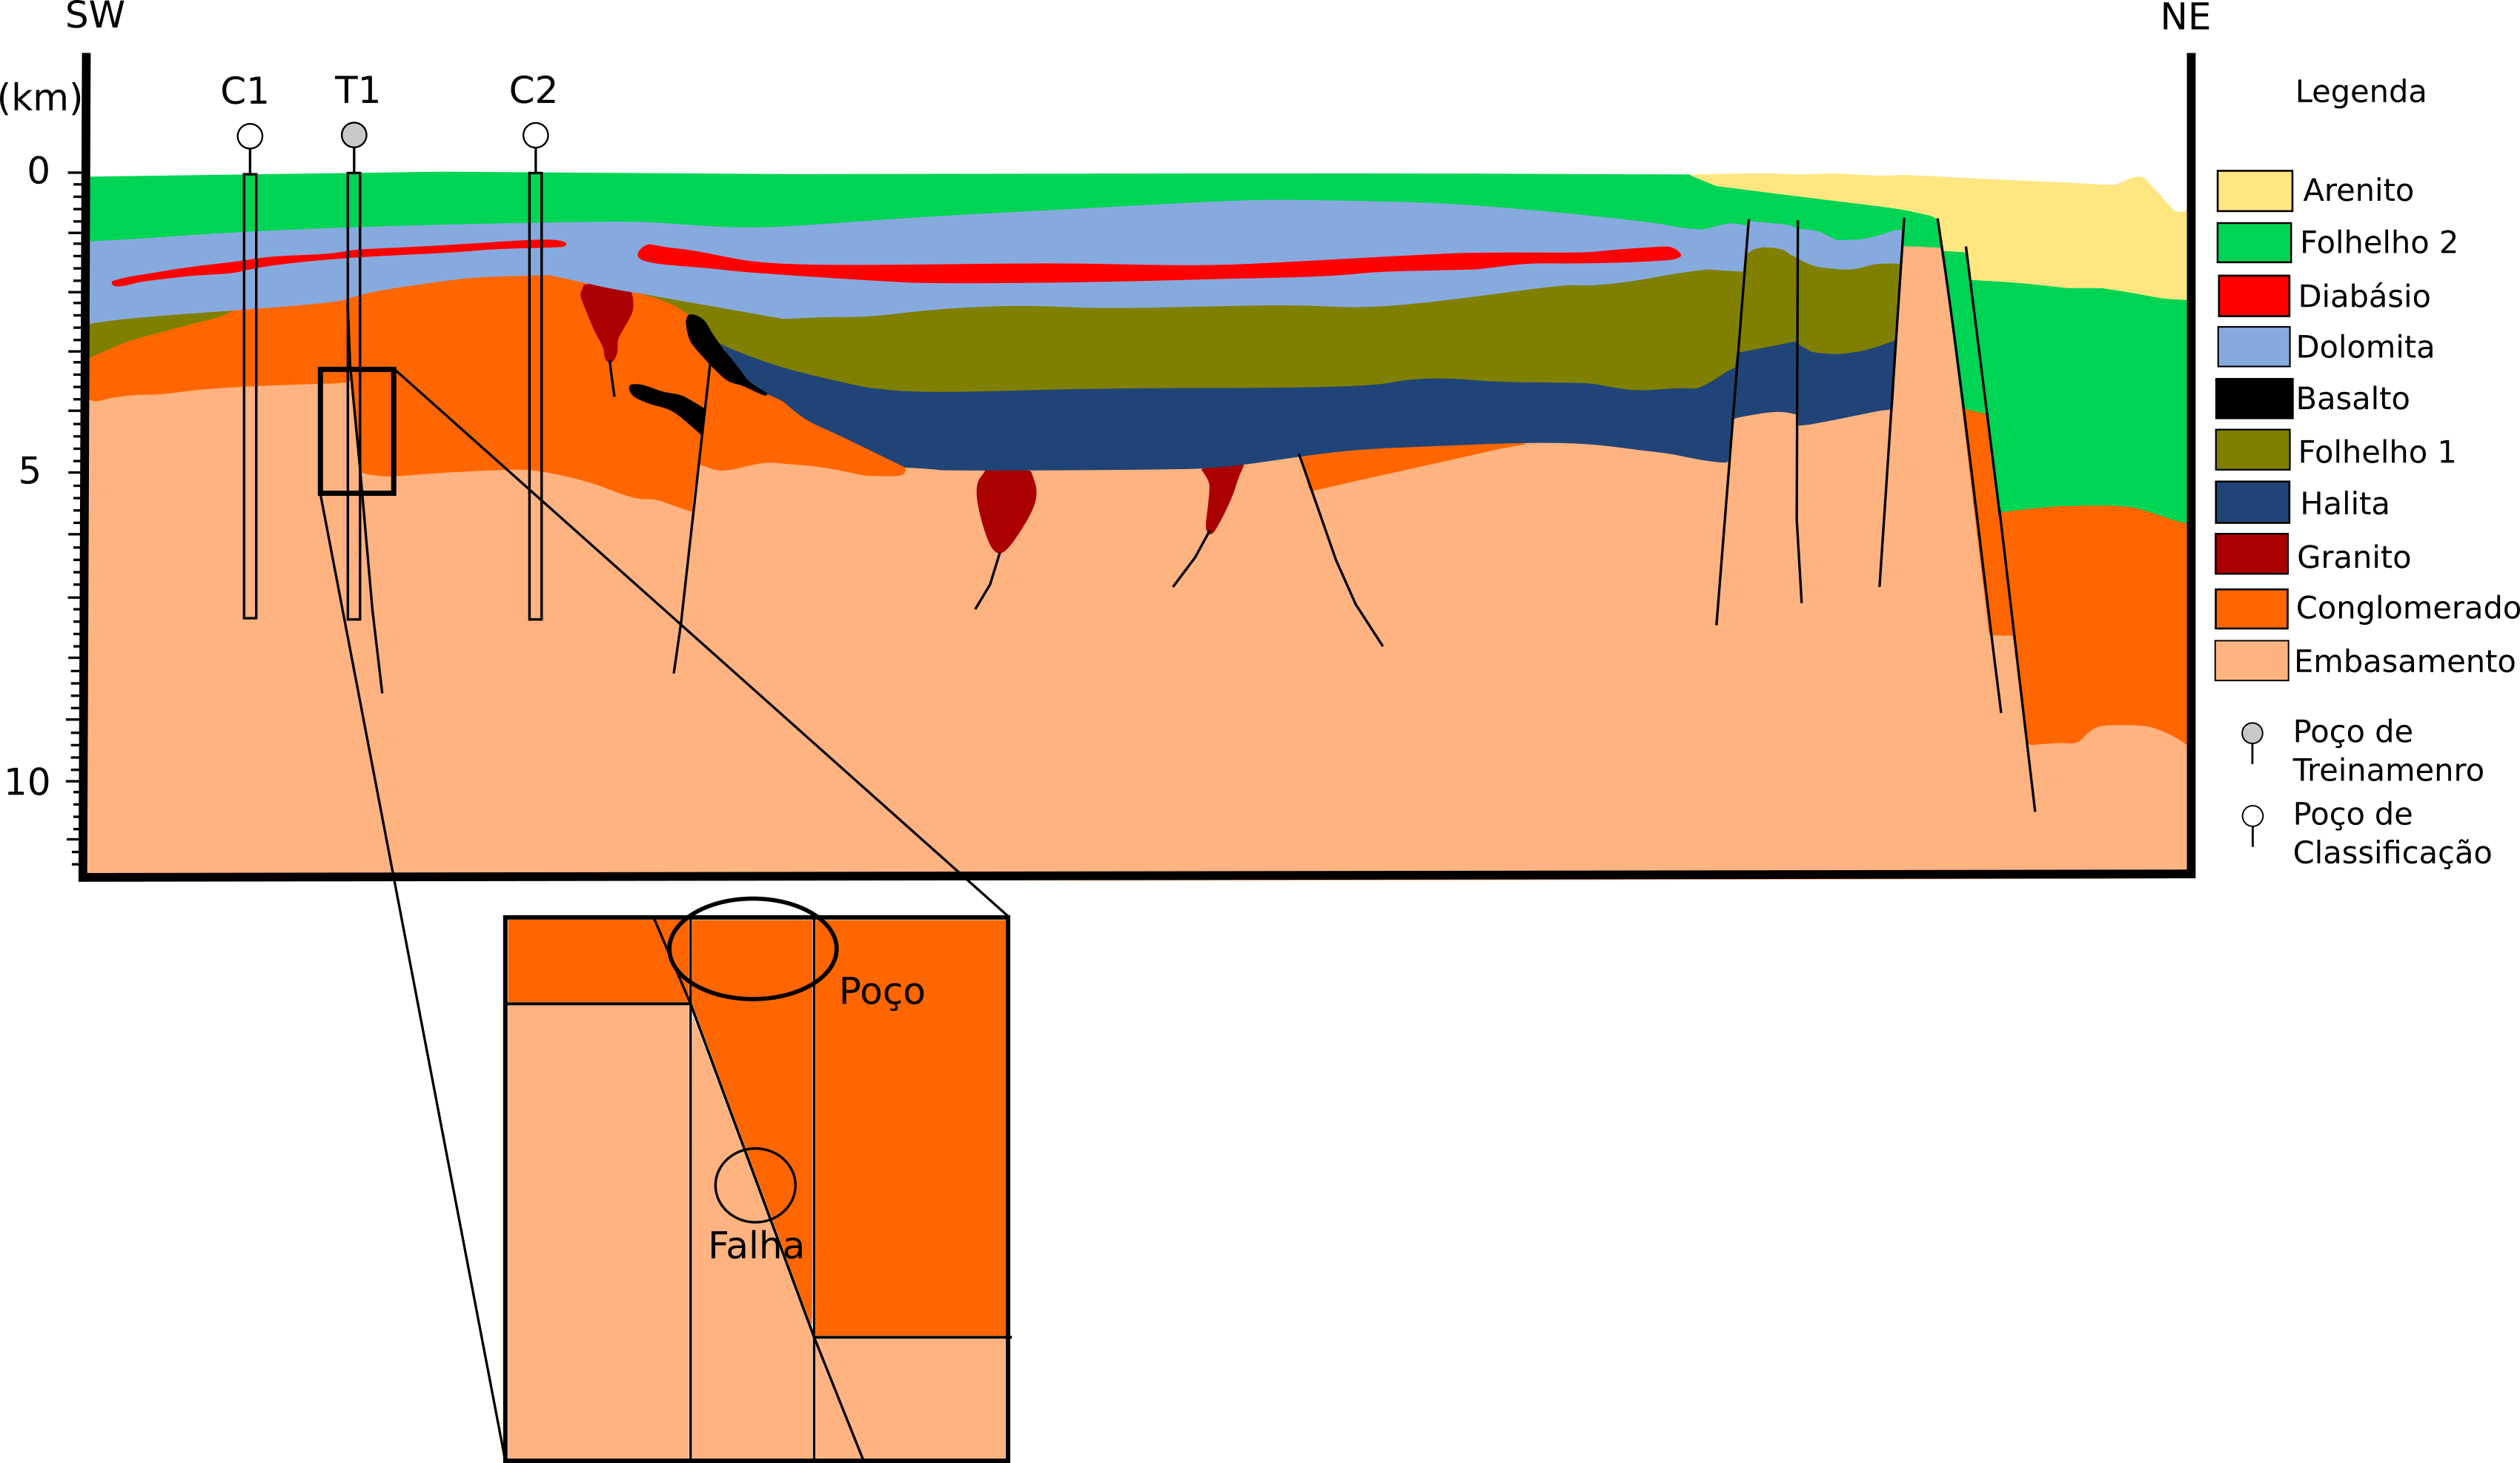
\includegraphics[scale=0.5]{Imagens/Modelo.png}
	}
	\caption{Modelo Simplificado baseado em \cite{Sal2008}.}
	\label{modelo}
\end{figure}

A partir da Fig. \ref{modelo} foram gerados três poços, na parte SW do perfil, com profundidades de $7$ km cada. Os três poços contém um conjunto com $4$ dados de propriedades físicas que são densidade, raio-gama, resistividade e velocidade, respectivamente. Os valores de propriedades físicas utilizados foram  baseados, em resultados já publicados, na literatura geocientífica, anteriormente, e retirados de \citet{Telford_1993}. Os poços simulam dados de \textit{well logging} com uma taxa de amostragem de $10$ m.

Os poços simulam diferentes padrões interpretativos usuais da ciência de perfilagem \footnote{Padrões usuais reconhecido por intérpretes geralmente associados a horizontes de interesse. Esses padrões são identificados como padrões sinos, sinos invertidos, serra e caixa.}. O poço denominado T$1$ \footnote{T$1$: poço escolhido para treinar a rede neuronal.} se localiza entre os poços C$1$ e C$2$ atravessando uma falha normal. 

A Fig. \ref{T1} apresenta os dados do poço T1. As espessuras das camadas são de $800$ m de embasamento, $2$ km de uma mistura crescente entre conglomerado e embasamento, perfazendo um padrão sino nos dados de perfilagem, $2$ km de conglomerado, $1$ km de dolomita (pacote inferior), $300$ m de diabásio, $400$ m de dolomita (pacote superior), $600$ m de folhelho $2$. A falha foi representada por uma função linear da variação de profundidade por propriedade física de uma mistura crescente de conglomerado e embasamento.

\begin{figure}[H]
	\centering
	\setlength{\fboxsep}{8pt}
	\setlength{\fboxrule}{0.1pt}
	\fbox{
		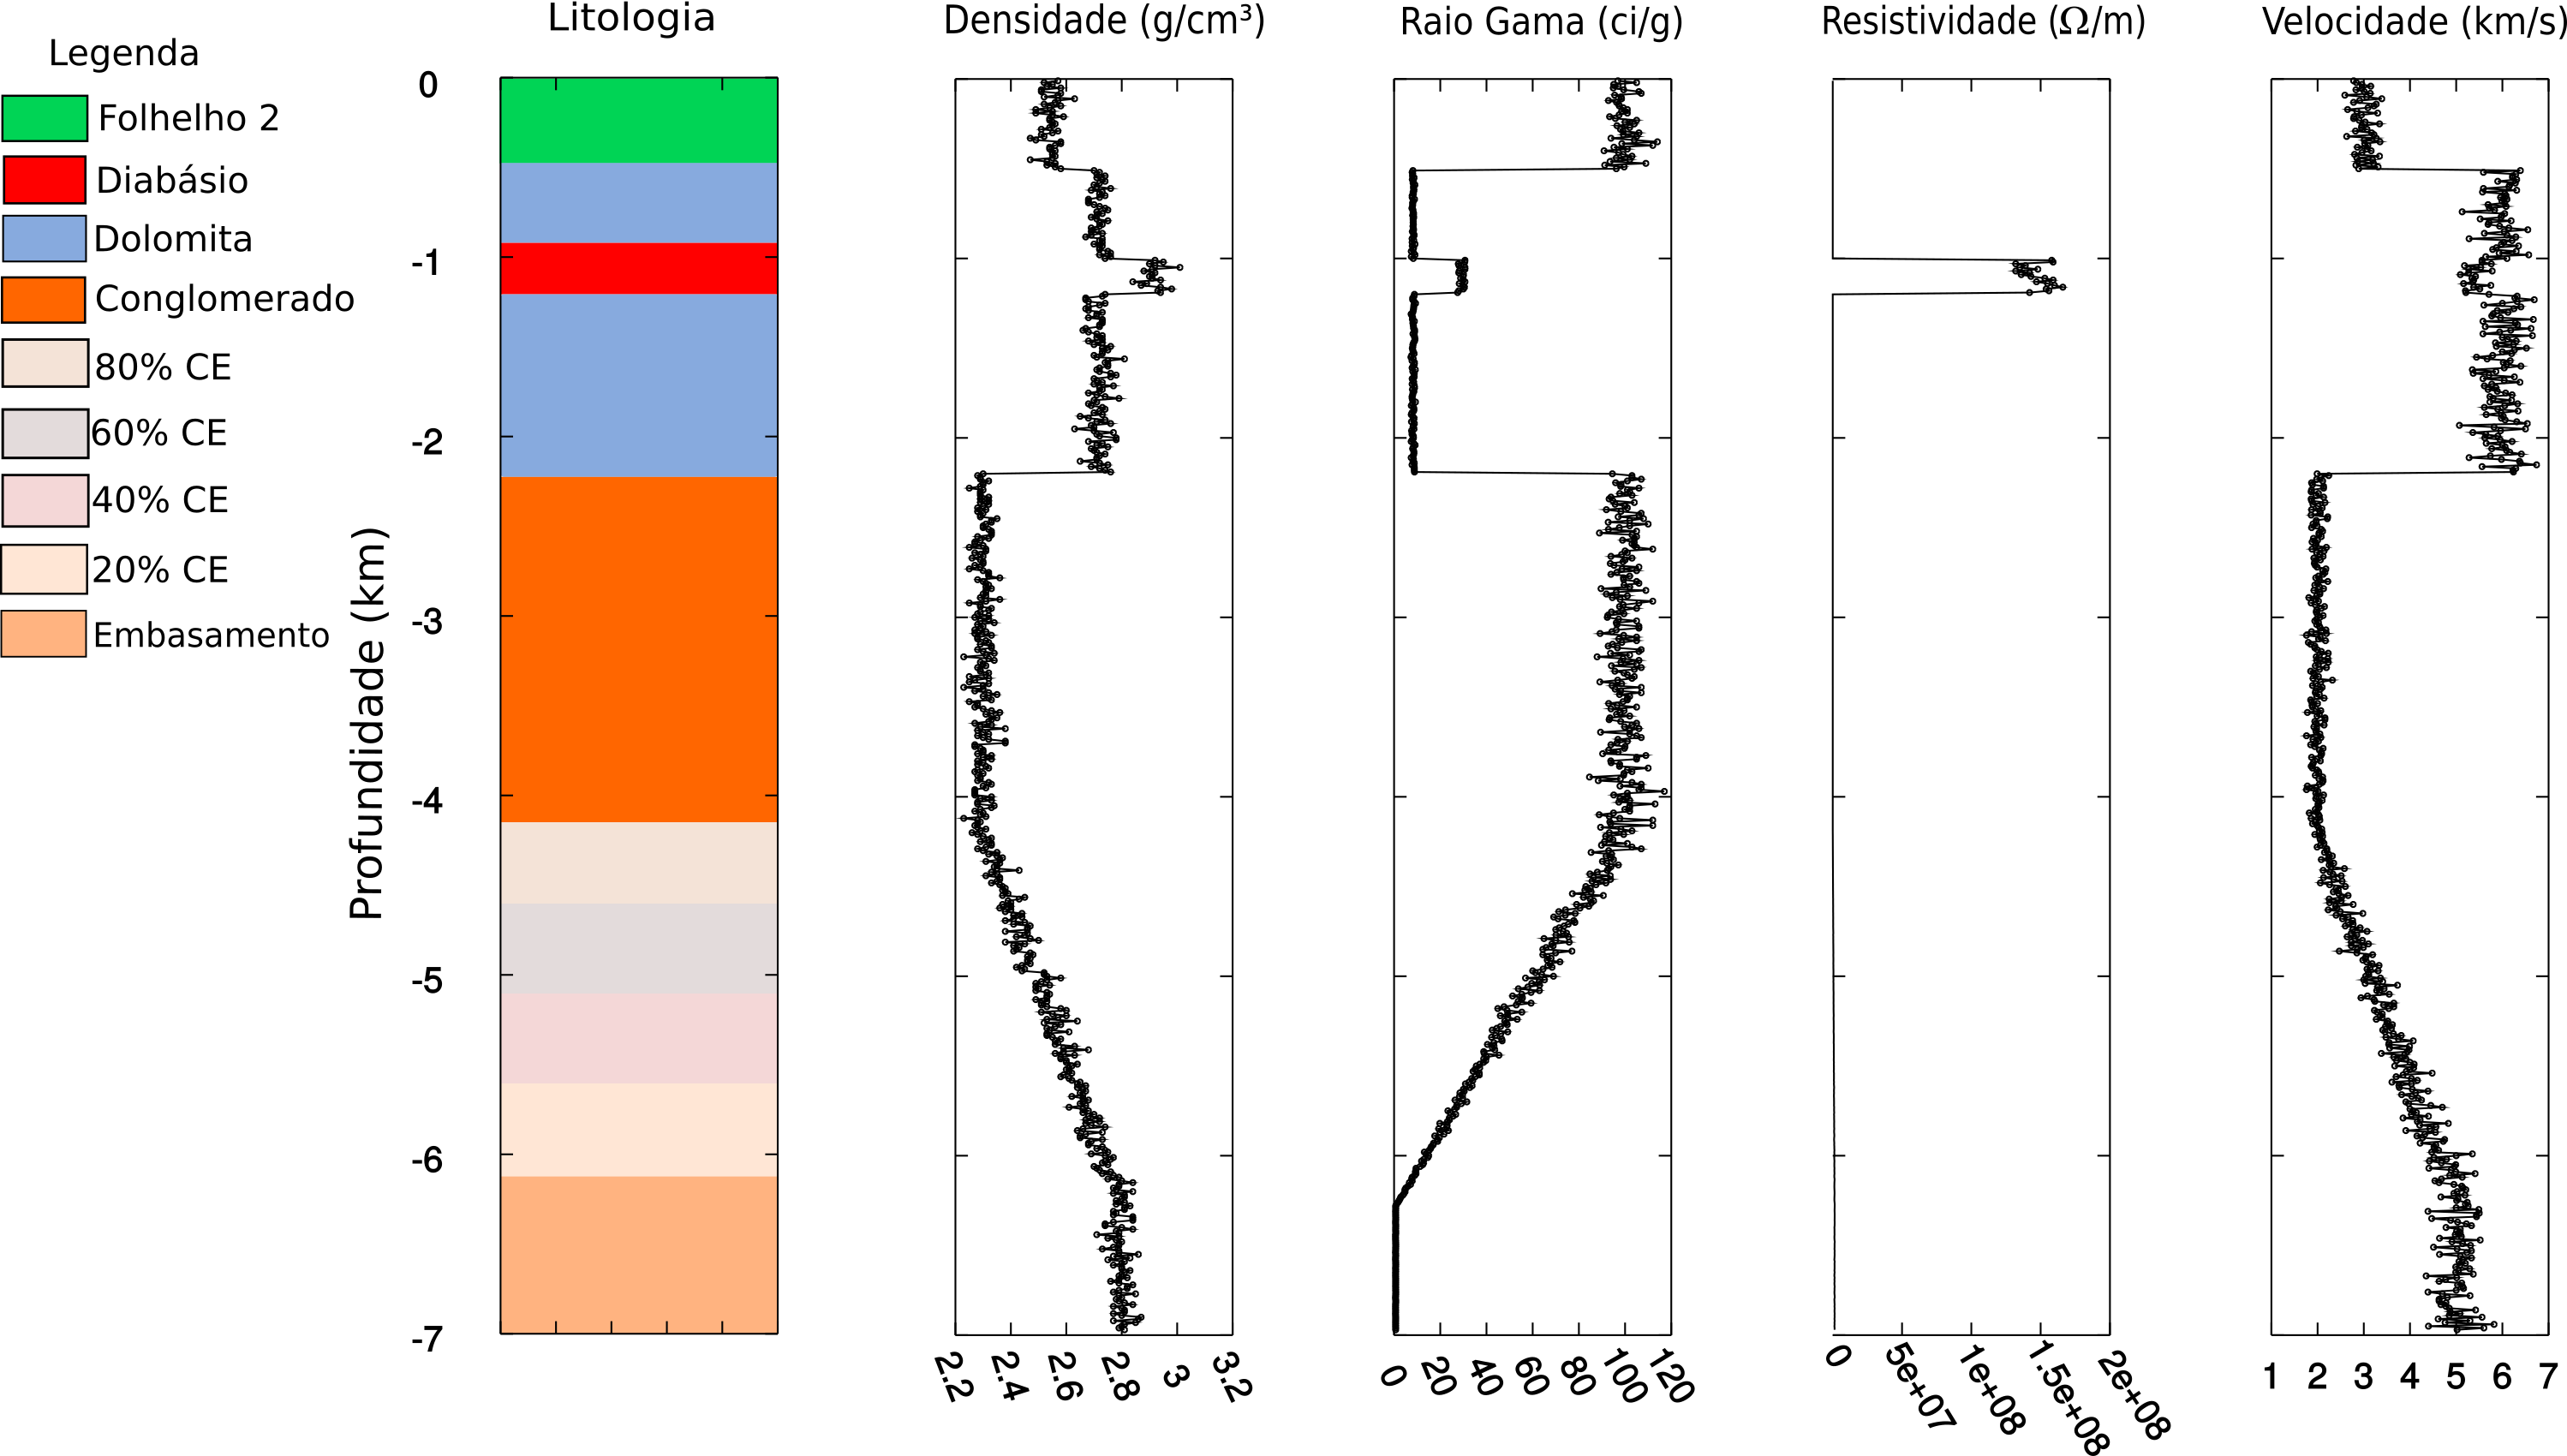
\includegraphics[scale=0.5]{Imagens/PocoT1.png}
	}
	\caption{Dado de perfilagem sintético, T1. Aonde a porcentagem de CE indica a mistura de conglomerado com embasamento}
	\label{T1}
\end{figure}

O poço C$1$\footnote{C1: Poço de classificação da rede neuronal número 1.}, Fig. \ref{C1}, possui as mesmas classes de rochas do poço T$1$. A escolha da posição dos poços quase que exclusivamente na parte SW do perfil se deu em virtude da localização do poço T$1$. Uma vez que espera-se da rede já treinada um reconhecimento das classes já estudadas. Os pacotes sedimentares apresentam espessuras de $2,8$ km de embasamento, $1,6$ km de conglomerado, $1$ km de dolomita (segundo pacote), $200$ m de diabásio, $500$ m de dolomita (primeiro pacote) e $500$ m de folhelho. 

\begin{figure}[H]
	\centering
	\setlength{\fboxsep}{8pt}
	\setlength{\fboxrule}{0.1pt}
	\fbox{
		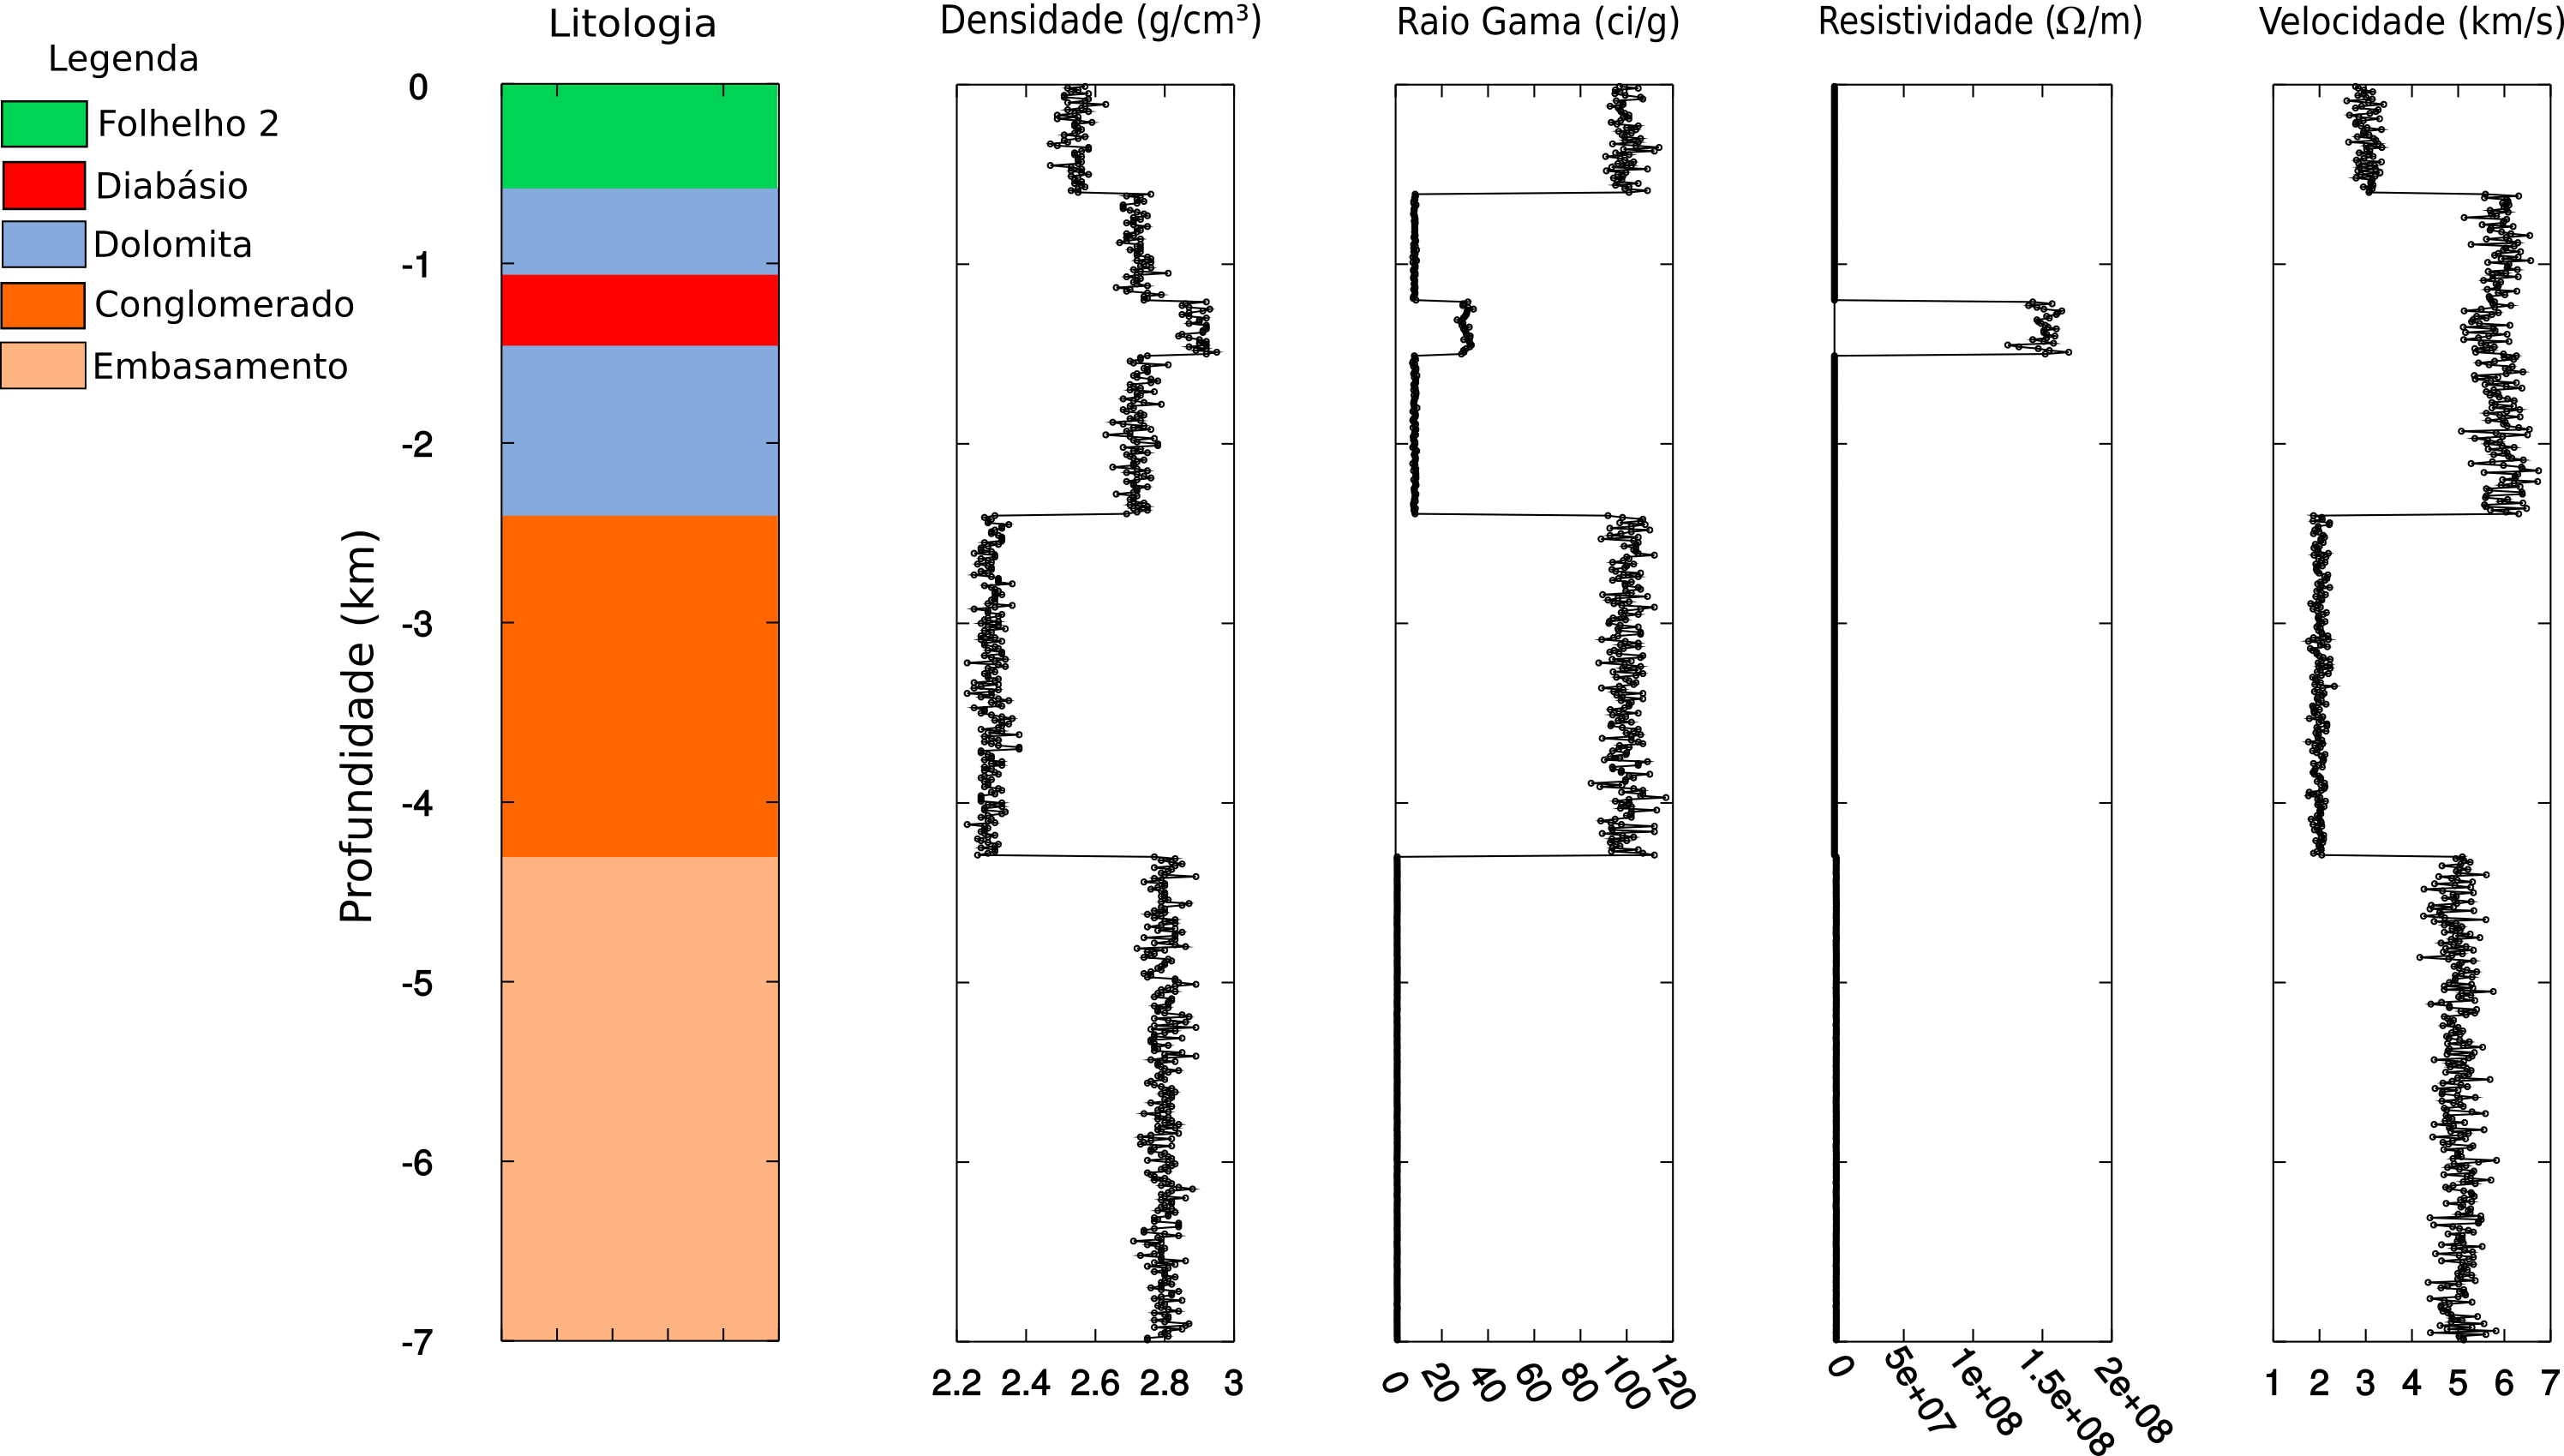
\includegraphics[scale=0.5]{Imagens/PocoC1.png}
	}
	\caption{Dado de perfilagem sintético, C1.}
	\label{C1}
\end{figure}

O poço C$2$\footnote{C2: Poço de classificação da rede neuronal número 2.}, Fig. \ref{C2}, localiza-se em um alto estrutural, e apresenta espessura de $5$ km de conglomerado. O embasamento possui uma espessura de $1,8$ km. Os pacotes de folhelho 2, dolomita (pacote superior) e diabásio $500$ m respectivamente. E o segundo pacote sedimentar de dolomita $1,6$ km.

\begin{figure}[H]
	\centering
	\setlength{\fboxsep}{8pt}
	\setlength{\fboxrule}{0.1pt}
	\fbox{
		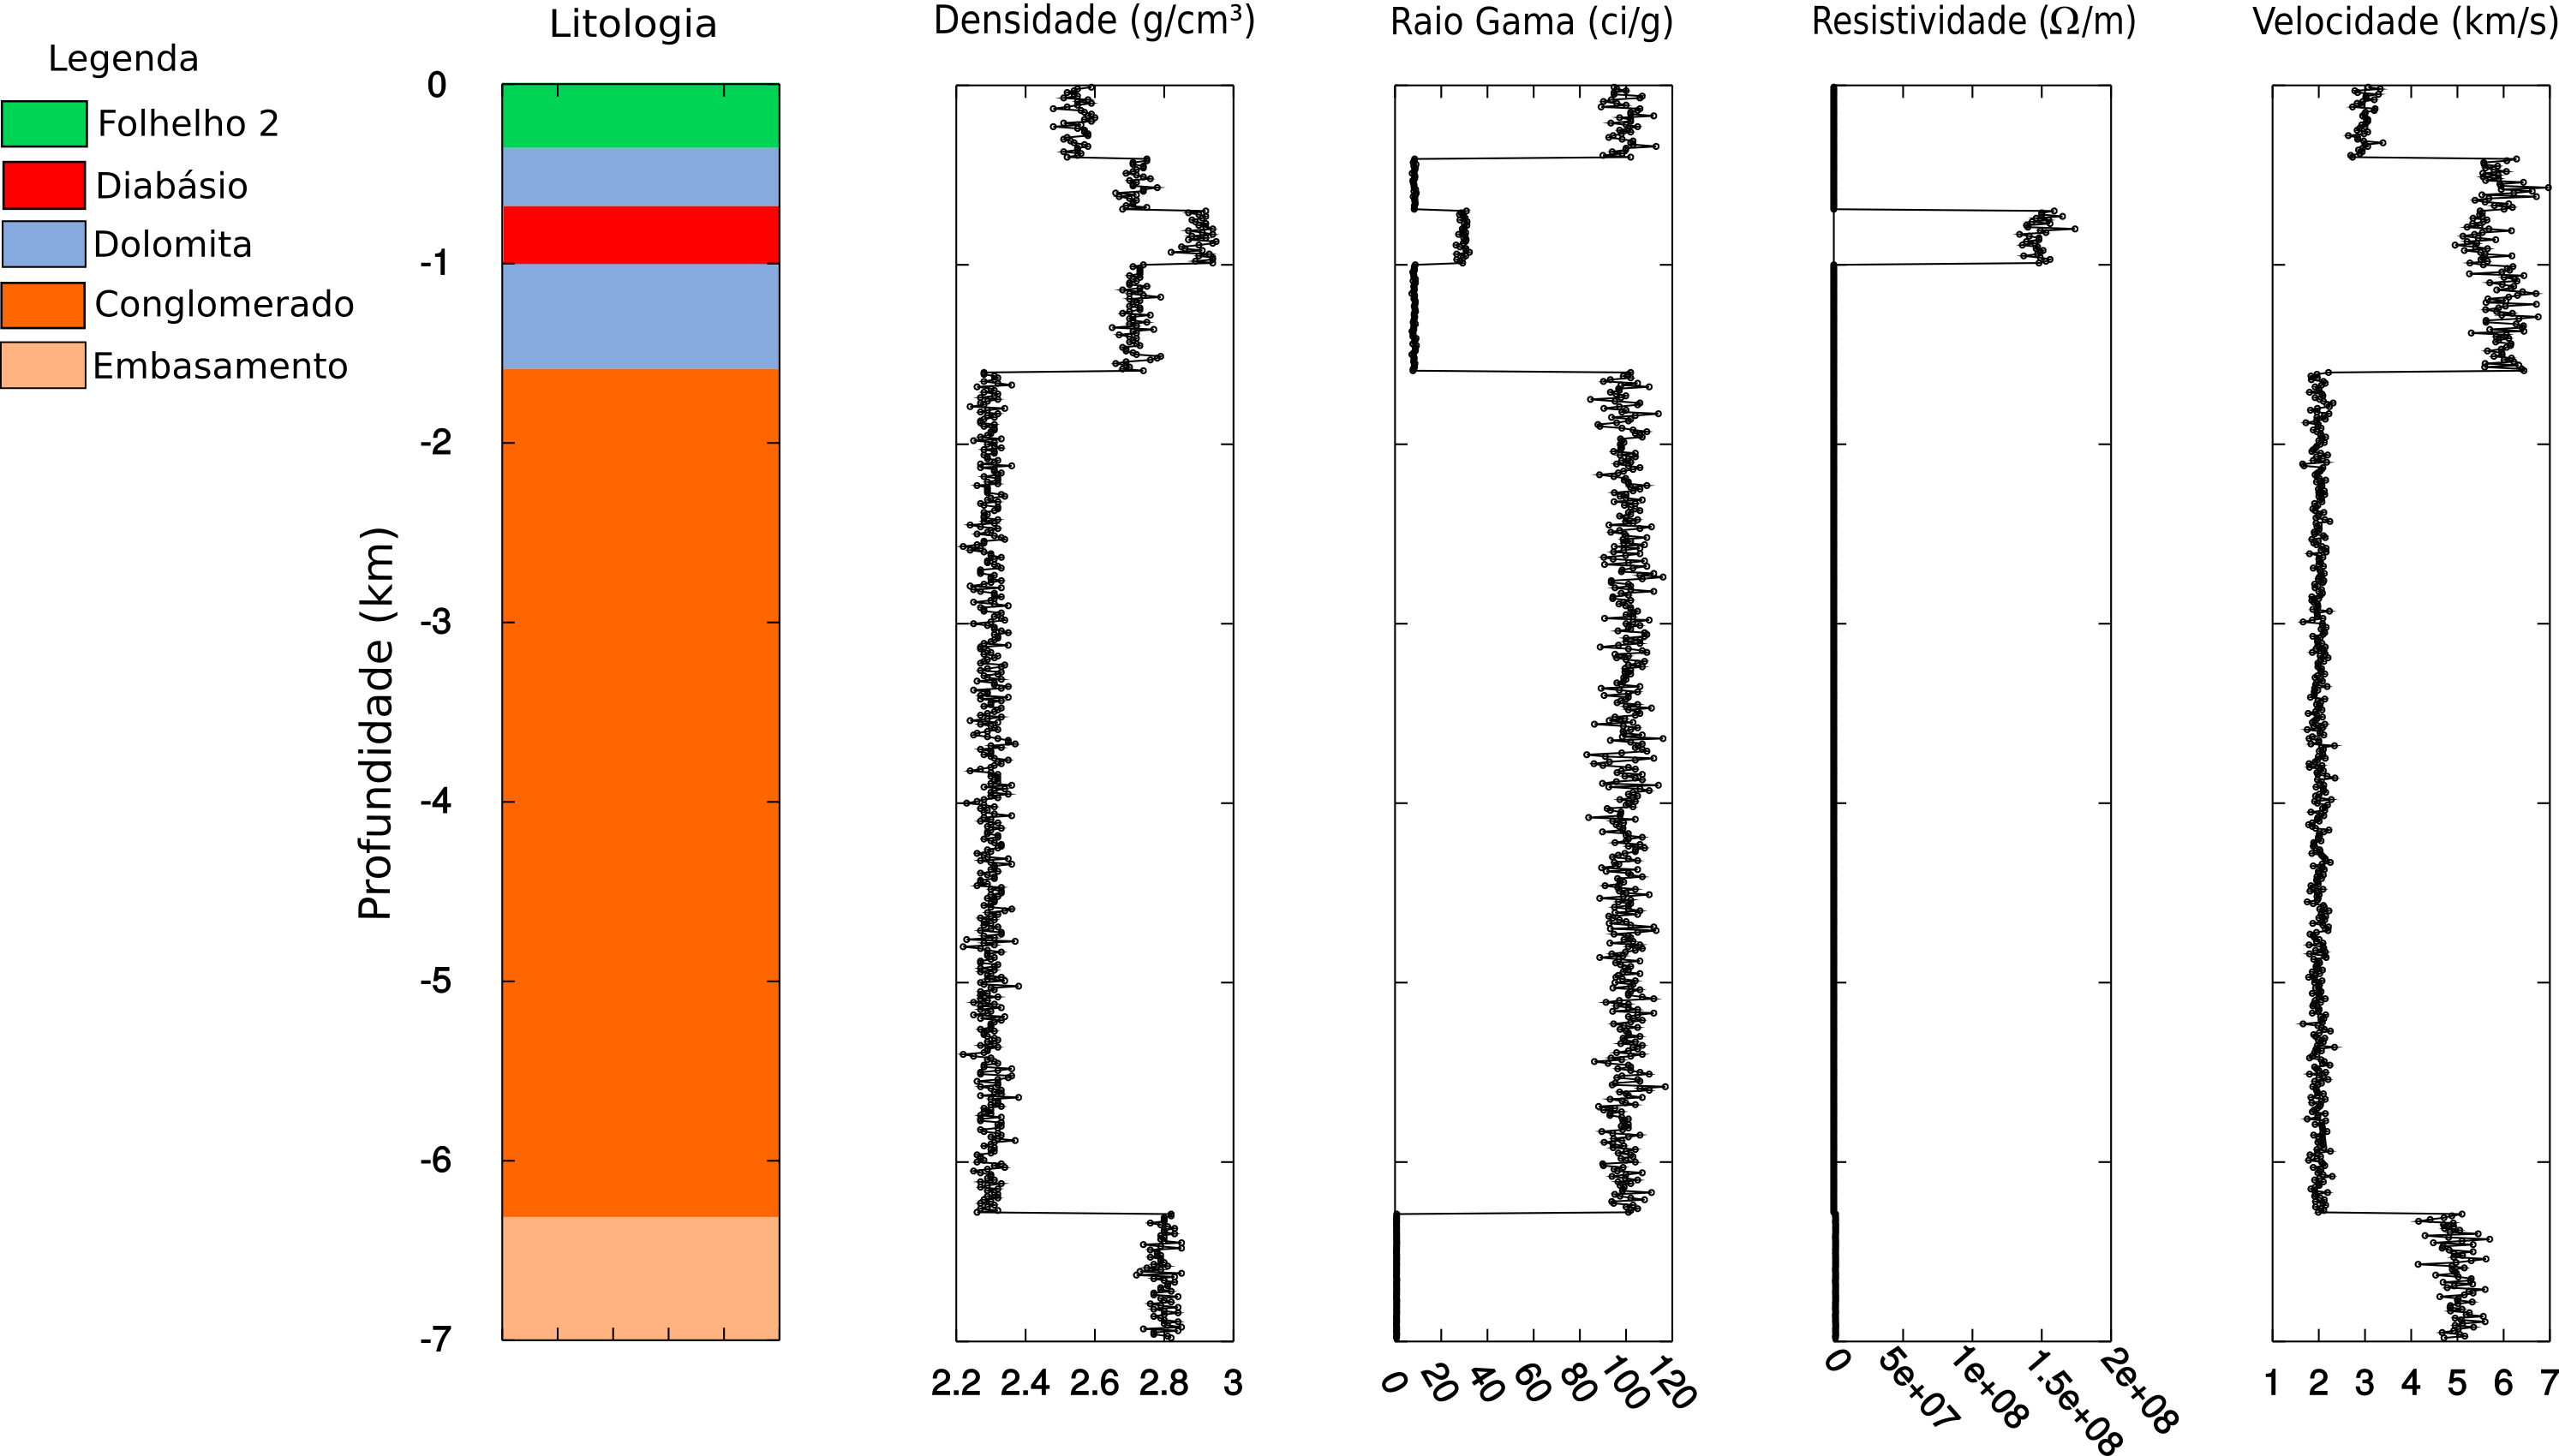
\includegraphics[scale=0.5]{Imagens/PocoC2.png}
	}
	\caption{Dado de perfilagem sintético, C2.}
	\label{C2}
\end{figure}

\section{Dado Real}

A triagem dos dados públicos contemplaram  $506$ arquivos *.dlis, $113$ *.lis, $118$ dados adicionais, $125$ perfis compostos digitalizados, $174$ poços públicos, $120$ arquivos *.agp, todos localizados na Bacia Sedimentar do Paraná. 

O conjunto de dados *.lis e *.dlis estão sendo convertidos para arquivos em formato texto, que serão posteriormente concatenados  com os arquivos *.agp afim de se obter o input da rede. Este processo ainda se encontra na fase inicial com cerca de $3\%$ concluído.

A Fig. \ref{real} mostra a localização e distribuição dos poços na Bacia do Paraná.

\begin{figure}[H]
	\centering
	\setlength{\fboxsep}{8pt}
	\setlength{\fboxrule}{0.1pt}
	\fbox{
		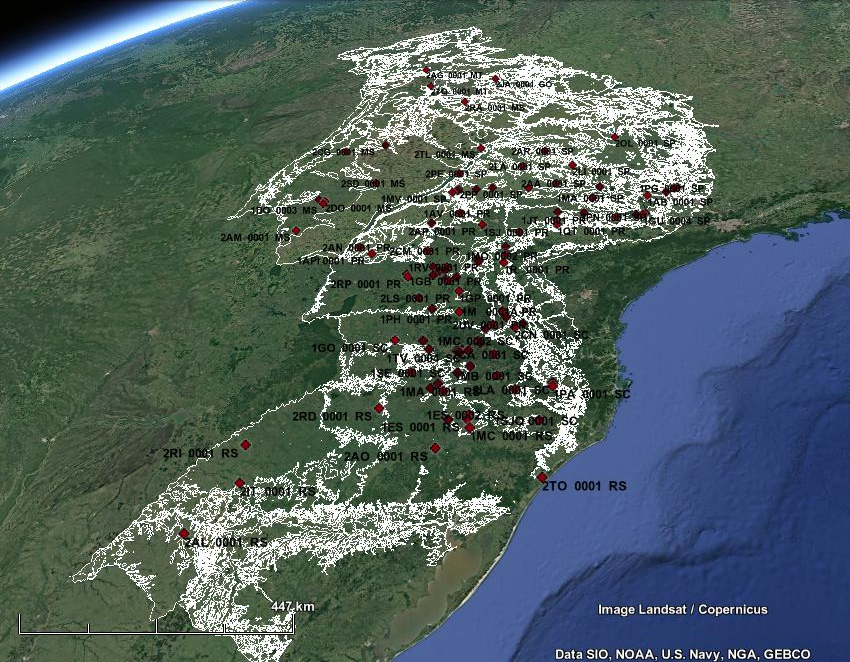
\includegraphics[scale=0.5]{Imagens/Pocos.jpg}
	}
	\caption{Localização do total de poços de trabalho.}
	\label{real}
\end{figure}

\subsection{Dados reais e treinamento e classificação da rede}

Como uma primeira abordagem com os dados reais foram escolhidos dois poços localizados na borda leste da Bacia Sedimentar do Paraná que preenchessem alguns pré-requisitos.

\begin{enumerate}
	\item Os primeiros poços devem estar localizados próximos para garantir um controle inicial no que tange as litologias presentes no poço de treinamento. 
	\item O poço de treinamento deve possuir a maior quantidade possível de dados por litologia
	\item As entradas da rede devem ser compostas das mesmas propriedades físicas
	\item As propriedades físicas que definem litologia devem ser priorizadas quando possível.
\end{enumerate}

O mapa da Fig. \ref{loc02} aponta a localização dos dois poços iniciais para o treinamento da rede.  


\begin{figure}[H]
	\flushleft
	\setlength{\fboxsep}{8pt}
	\setlength{\fboxrule}{0.1pt}
	\fbox{
		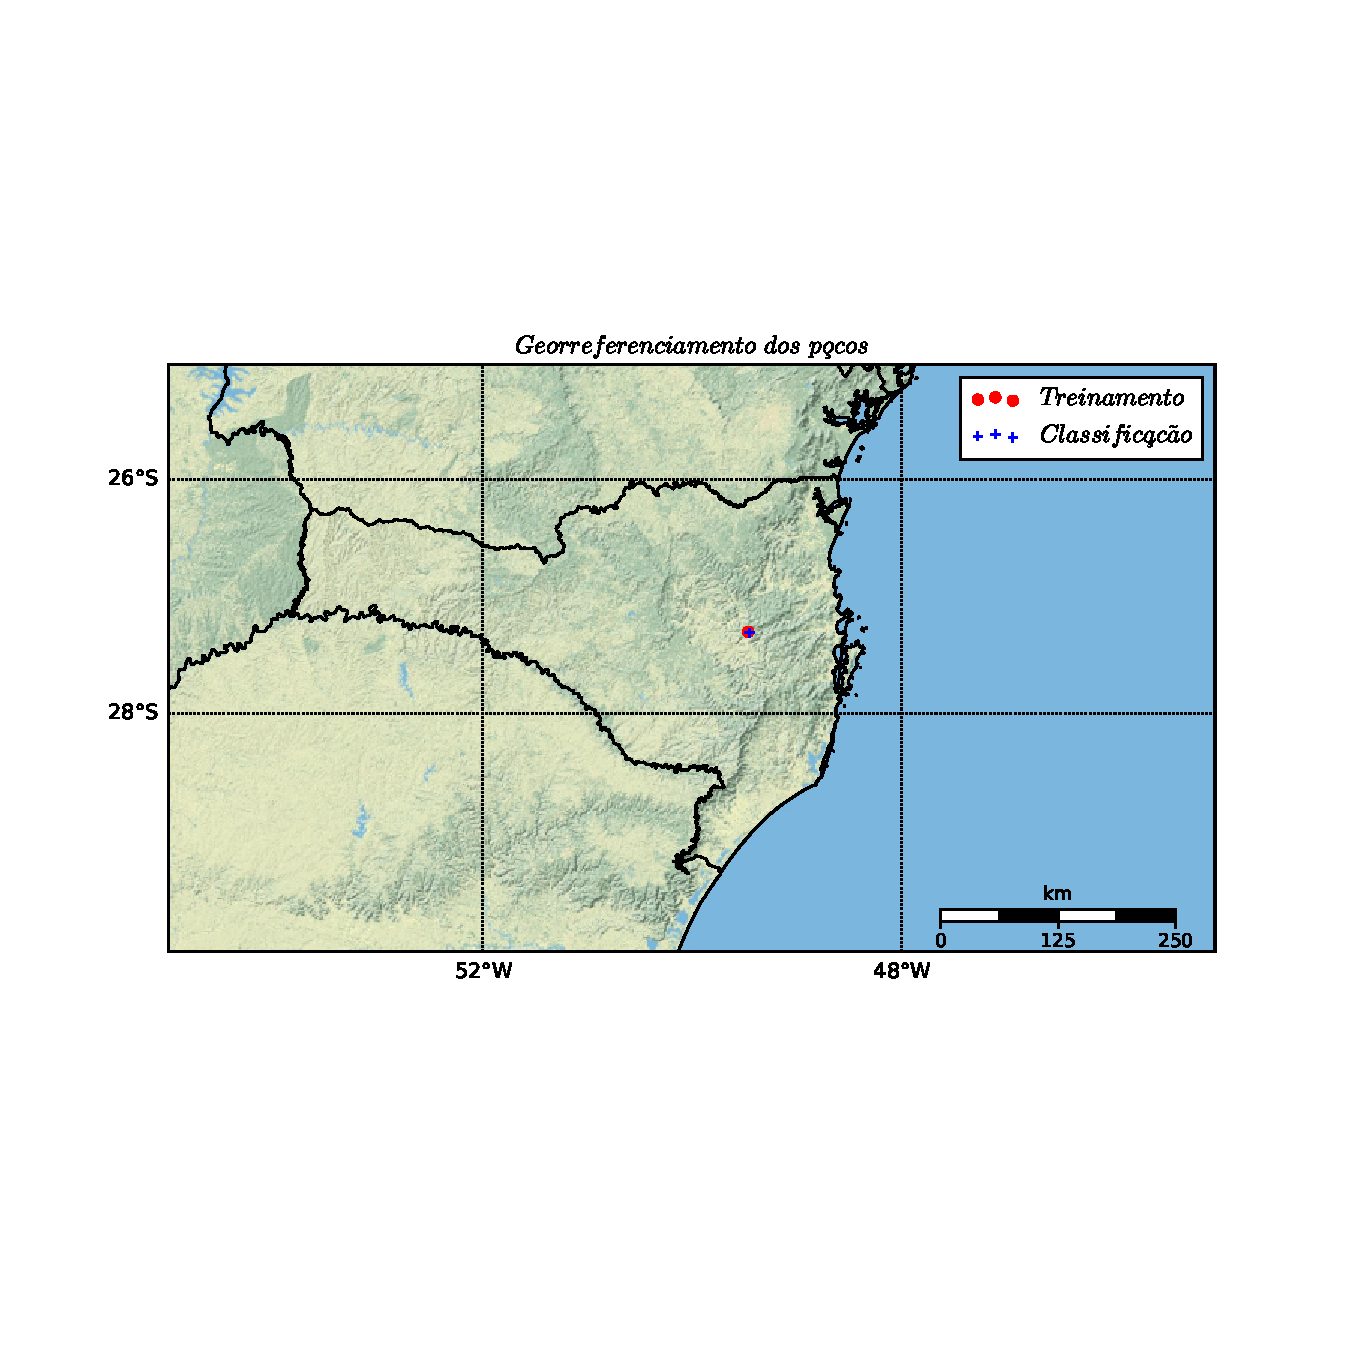
\includegraphics[scale=0.8]{Imagens/locmap02.pdf}
	}
	\caption{Localização dos poços escolhidos.}
	\label{loc02}
\end{figure}

O primeiro poço escolhido para o treinamento da rede foi o de nome 1BN0001SC localizado na borda leste da Bacia Sedimentar do Paraná no Estado de Santa Catarina. A taxa de amostragem é $0,2$ medidas por metro e possui uma profundidade de aproximadamente $1400$ m.  As propriedades medidas foram o potencial espontâneo, raios-gama, resistividade lateral, radiação neutrônica além de medidas de propriedades para inferência da qualidade do poço e medidas de complementação a perfis sísmicos tais como \textit{Transient Time Integrator}.  

O segundo poço denomina-se 1BN0002SC e foi perfurado a poucos quilômetros de distância ao sul do poço de treinamento. Possui uma profundidade de $700$ m e taxa de amostragem no valor de $0,2$ medidas por metro. As propriedades inferidas foram Potencial espontâneo, resistividade lateral, densidade de formação, raio-gama, além de medidas de propriedades para inferência da qualidade do poço e medidas de complementação a perfis sísmicos tais como \textit{Integral Time Travel}. 

Foram inicialmente escolhidas quatro propriedades que são comuns em ambos os poços dentre as quais podem-se destacar o potencial espontâneo, resitividade lateral, TTI, TOT. As Figuras \ref{1BN0002SCa} e \ref{1BN0002SCb} apresentam a distribuição de propriedades físicas relacionadas com a litologia associado à variação de profundidade, respectivamente. 


\begin{figure}[H]
	\centering
	\subfigure{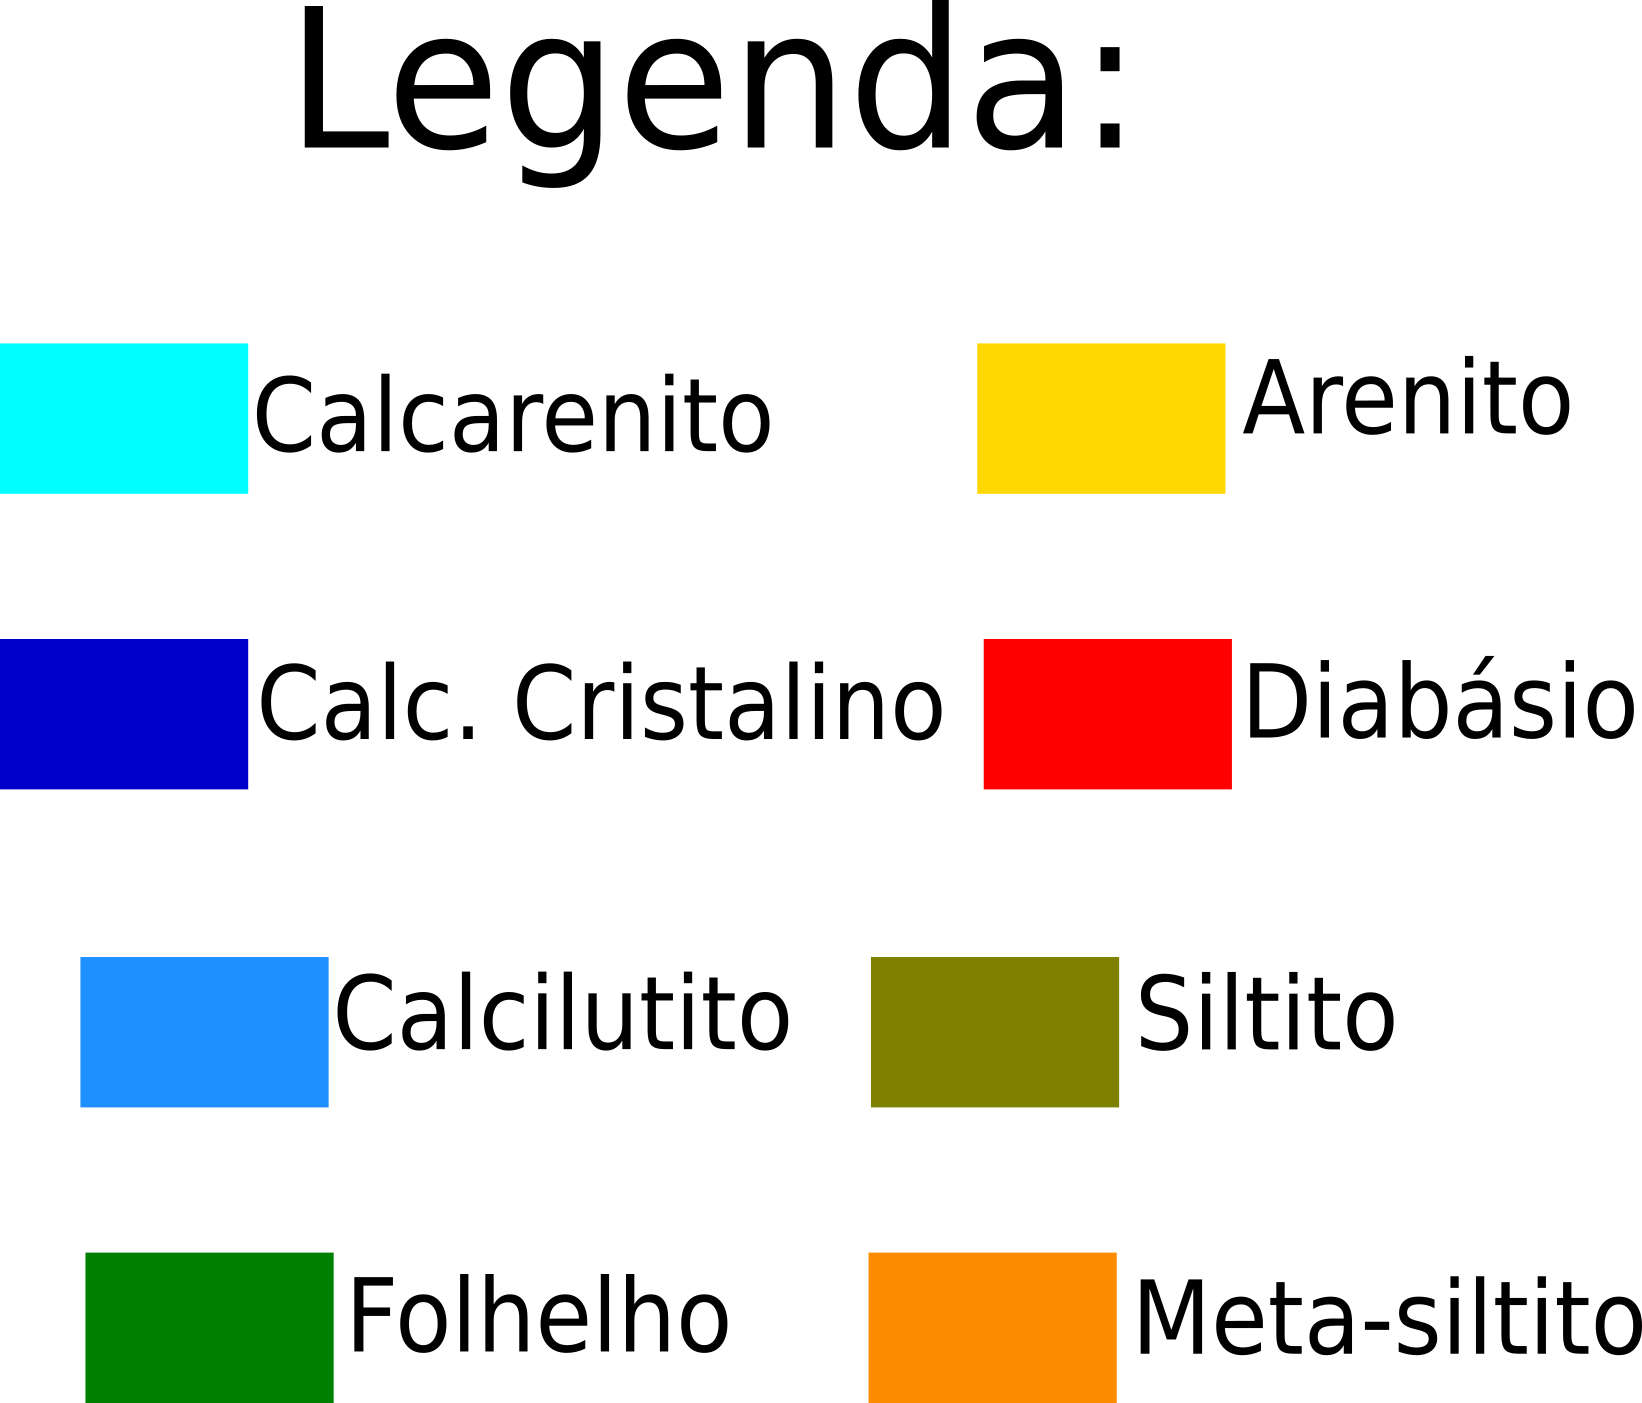
\includegraphics[width=2.5cm, height=2.5cm]{Imagens/legenda.png}}
	\qquad                                                           
	\subfigure[ref1][Litologia]{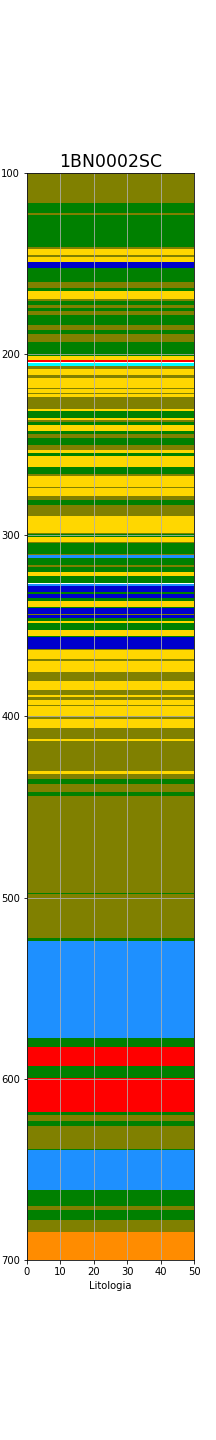
\includegraphics[width=2.8cm, height=12cm]{Imagens/1BN0002SC_lit2.png}}
	\qquad                                                             
	\subfigure[ref2][SP]{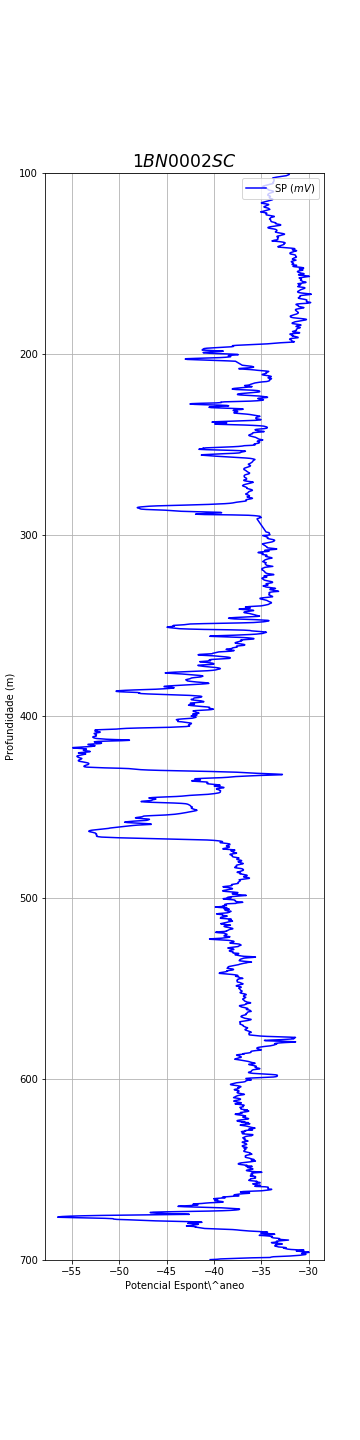
\includegraphics[width=3.0cm]{Imagens/1BN0002SC_SP.png}}
	\qquad
	\subfigure[ref3][RLAT]{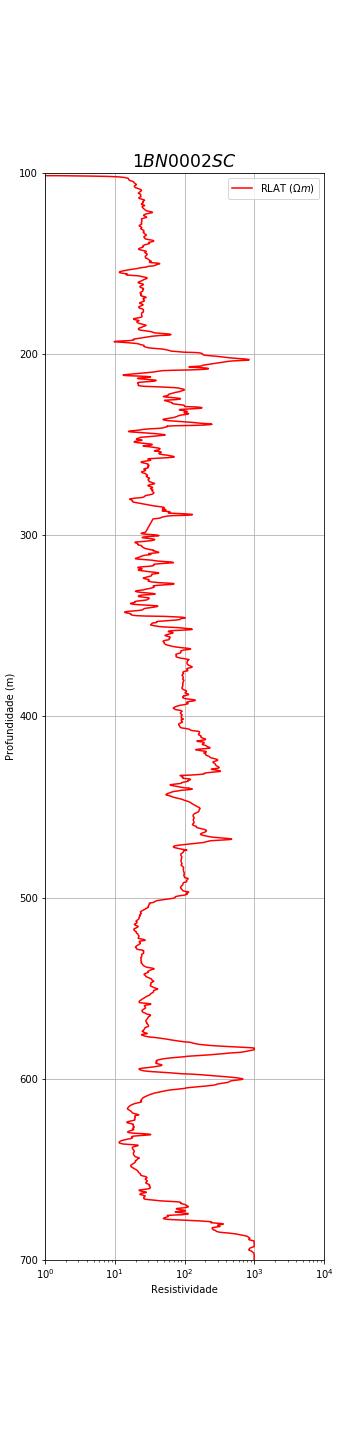
\includegraphics[width=3.0cm]{Imagens/1BN0002SC_res.png}}
	\qquad
	\caption{Poço 1BN0002SC e as respectivas propriedades físicas escolhidas para o teste. Em (b) tem-se a variação de litologia com a profundidade, (c) o potencial espontâneo e em (d) a resistividade lateral.   } 
	\label{1BN0002SCa}
\end{figure}


\begin{figure}[H]
	\centering                                                         
    \subfigure{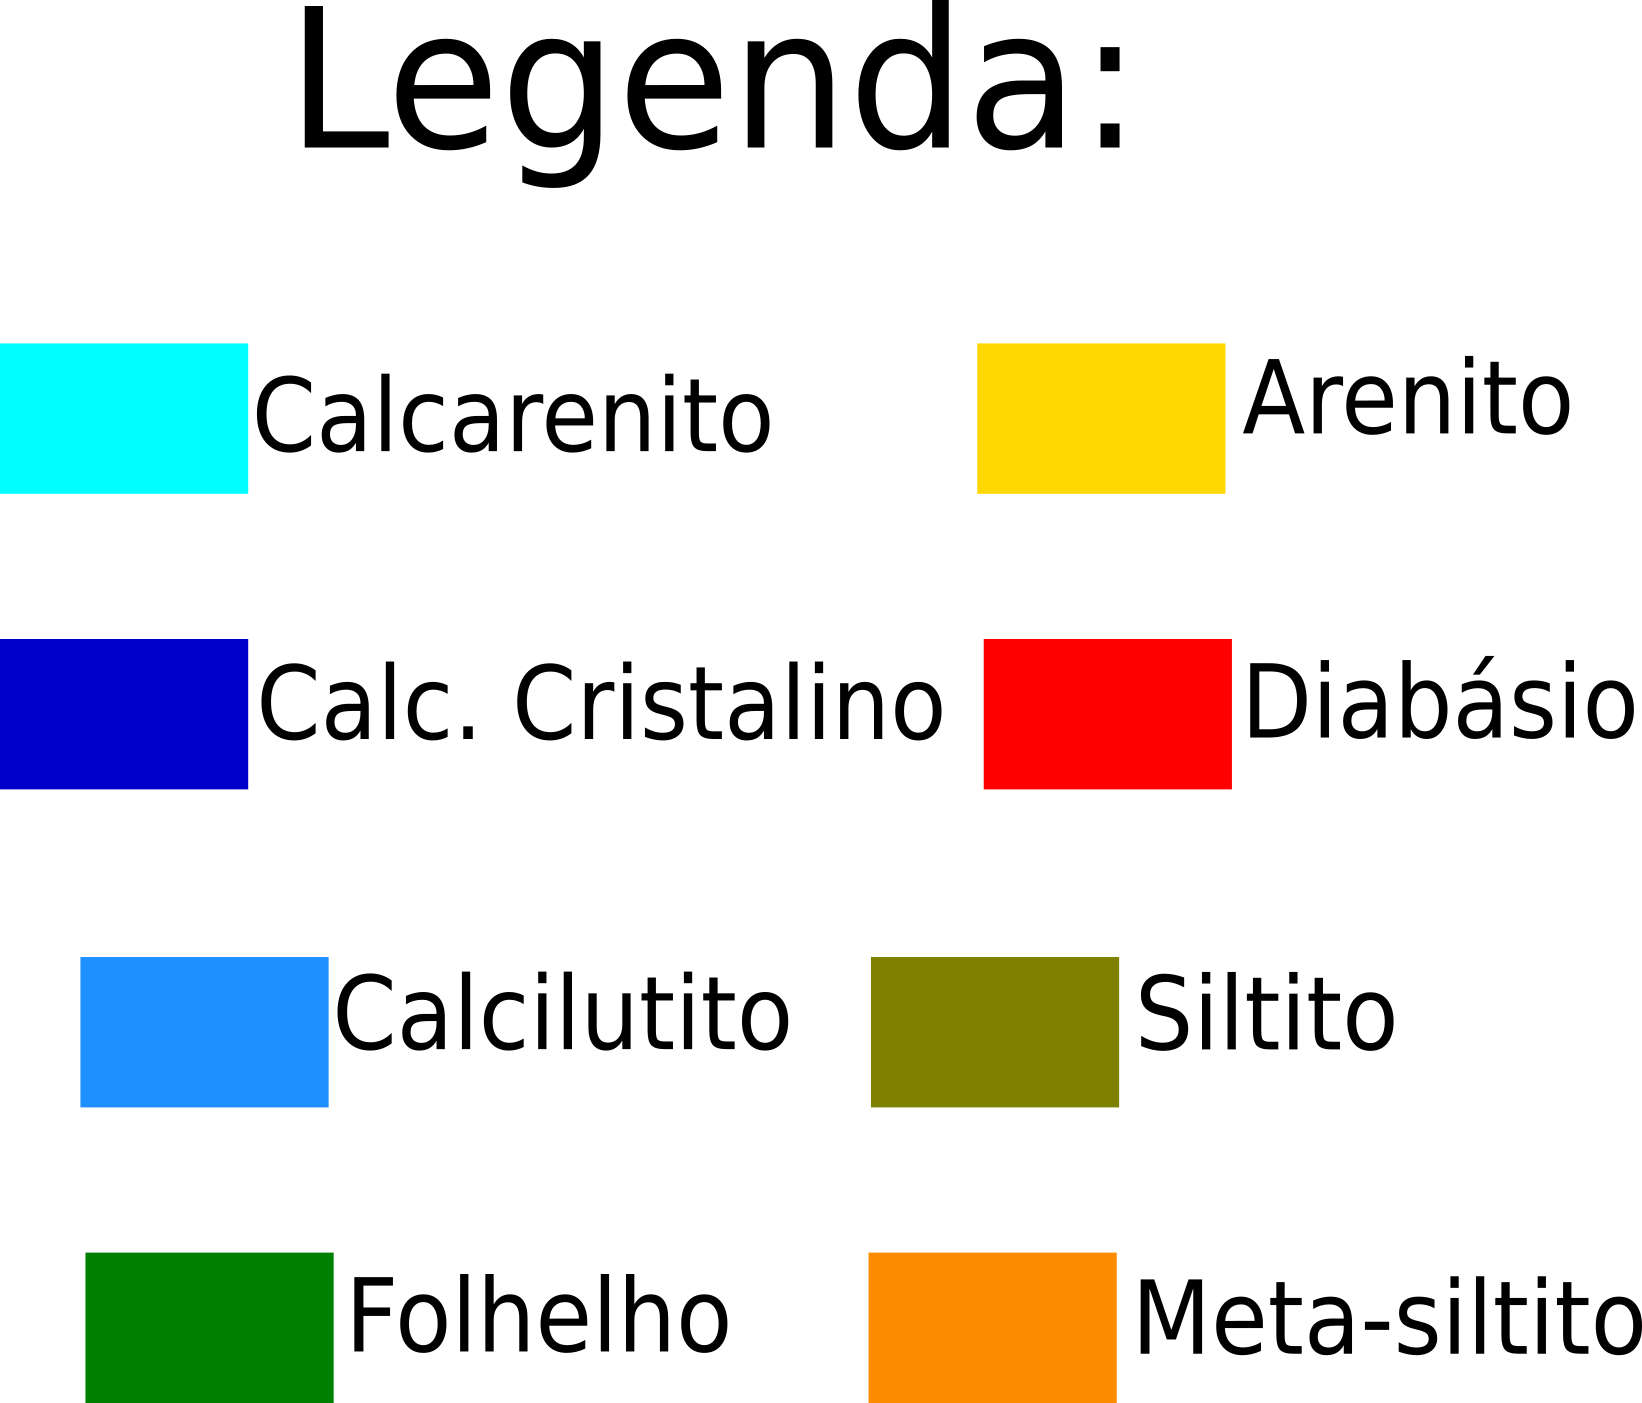
\includegraphics[width=2.5cm, height=2.5cm]{Imagens/legenda.png}}
    \qquad                                                           
    \subfigure[ref1][Litologia]{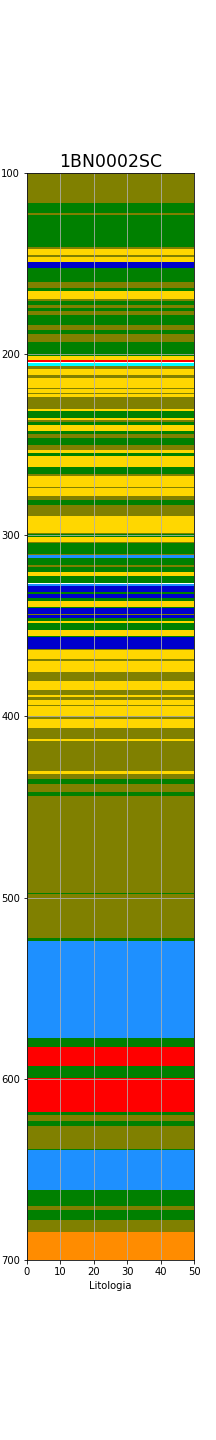
\includegraphics[width=2.8cm, height=12cm]{Imagens/1BN0002SC_lit2.png}}
    \qquad                                                             
	\subfigure[ref4][TTI]{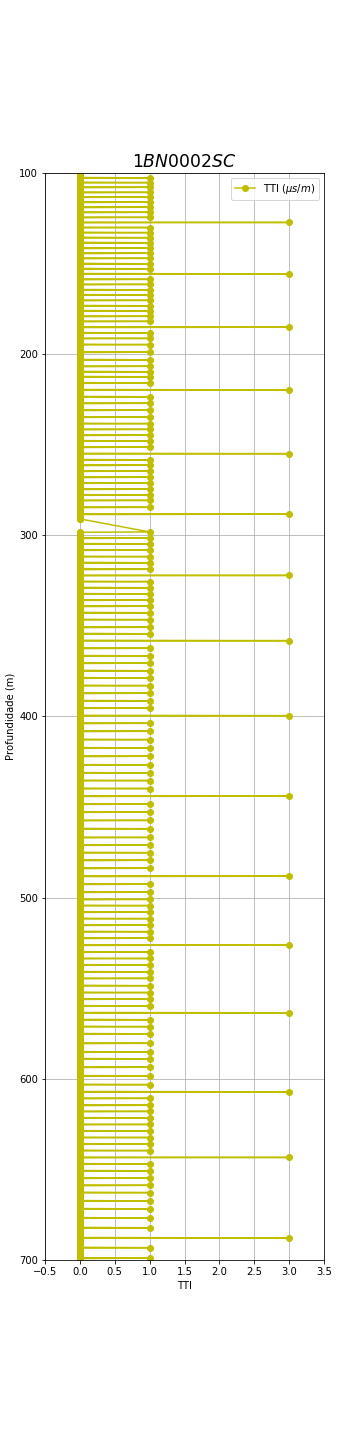
\includegraphics[width=3.0cm]{Imagens/1BN0002SC_TTI.png}}
	\qquad
	\subfigure[ref5][TOT]{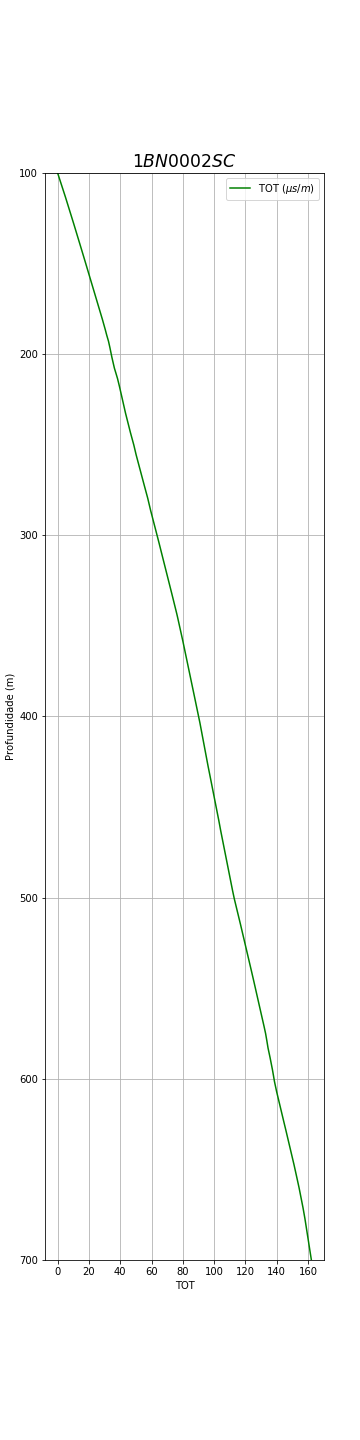
\includegraphics[width=3.0cm]{Imagens/1BN0002SC_TOT.png}}
	\qquad
	\caption{Poço 1BN0002SC e as respectivas propriedades físicas escolhidas para o teste. Em (b) tem-se a variação de litologia com a profundidade, (c) \textit{Transient Time Integrator} e em (d) TOT.}
	\label{1BN0002SCb}
\end{figure}

Muito embora o critério de escolha dos poços tenham sido obedecidos alumas litologias presentes no poço de classificação não existem no poço de treinamento. Isso torna necessário que futuramente seja criado um banco de dados para classificação de rochas que contenham dados de propriedades que sejam independentes da profundidade. Extinguindo-se o conceito poço de treinamento substituindo-o por Banco de dados litológicos. 
   


  \chapter{Resultados esperados}

  \chapter{Conclusões}

O teste de convergência da rede, Fig \ref{convergencia}, realizado durante a etapa de treinamento, indicou que o número de erros não iria diminuir após o milésimo ciclo de treinamento. Sendo o resultado, Fig. \ref{SOM}, deste teste usado como parâmetro para o número de repetições realizadas para os casos de identificação da rede. 

Os diagramas de velocidades por densidade e o de velocidade por raio-gama, Fig. \ref{clusterT1}, Fig. \ref{clusterC1} e Fig. \ref{clusterC2}, apresentaram os agrupamentos mais bem separados. Portanto estas propriedades físicas (densidade, velocidade e raio-gama) tem uma importância relativa maior ,na classificação das litologias dos poços C$1$ e C$2$. 

A saída da rede aponta que o maior caso de erros ocorreram em uma única classe de rocha, a do embasamento. Esses erros fizeram com que conglomerados fossem classificados como rochas do embasamento, nos dois casos dos poços de classificação, o poço C$1$ e o poço C$2$.  Uma das razões pode ser o fato das misturas de conglomerado e embasamento serem finas demais para a rede conseguir realizar uma identificação de padrão. Ou pelo fato dos conjuntos de propriedades físicas da mistura de $20\%$ se aproximar das propriedades físicas que representam o litotipo embasamento. 

O menor número de erros relativos encontrados, no poço C$2$, Fig. \ref{Class C2}, deve-se a escolha da alocação do furo, no perfil. O poço C$2$ localiza-se em um baixo estrutural, atingindo menos de $1$km do embasamento. Entretanto, o poço C$1$, Fig. \ref{Class C1}, encontra-se em um alto estrutural, divergindo do poço C$2$ e produzindo, consequentemente, os maiores erros relativos encontrados.    

O classificador de Euclides apresentou mais erros do que a rede neuronal de Kohonen com $42$ erros para o poço C$1$ e $12$ erros para o poço C$2$. E o classificador de Mahalanobis apresentou o resultado de identificação de poços com os maiores erros $79$ e $128$ respectivamente para os poços C$1$ e C$2$. 

Tal desempenho dos classificadores se deu por conta da existência de uma falha normal aonde foi escolhida a alocação do furo, Fig. \ref{modelo}. Nesta situação simulada há uma mistura entre os clusters em todos os espaços bi-dimensionais de propriedades analisadas tanto para o conglomerado quanto para o embasamento cristalino, Fig. \ref{clusterT1}. Portanto a definição dos centroides dos agrupamentos de propriedades ficam longe das distribuições ideais preditas no teste analítico do capítulo \ref{introducao}, na seção \ref{teste}.  

No tocante ao dado real, foram realizados seis testes com o objetivo de observar o comportamento da rede neuronal. Os dados que compõe a função que descreve a litologia para a rede é composta pelas seguintes entradas: SP, RLAT, TTI, TOT. Confirme indicado nas figuras \ref{1BN0002SCa} e \ref{1BN0002SCb} respectivamente. Essas entradas foram escolhidas de acordo com a disponibilidade de dados presentes nos poços de treinamento e classificação. A escolha de ambos os poços obedeceram o critério de proximidade entre si. Dado a alta amostragem presentes em ambos o poços optou-se por aumentar o número de neurônios da rede nos primeiros testes.

Os mapas auto-organizáveis concernentes ao teste $01$ indicam que a rede não consegue aprender a identificar os tipos litológicos presentes no poço de treinamento. Esse indicativo é apontado pela maior área dedicada a identificação de somente uma rocha, especificamente o calcilutito (vide figura \ref{SOMt01}) em detrimento as demais rochas. Em contrapartida, a convergência indica que a rede está aprendendo conforme indicado na figura \ref{Conv01}. Esse comportamento é justificado pelo número de épocas empregadas no presente teste. É importante ressaltar que, conforme apresentado na tabela \ref{Estatistica do teste $01$}, apenas $976$ neurônios são utilizados na etapa de identificação da rede, indicando um subaproveitamento de neurônios. A fase de identificação da rede indicou um erro de $2229$ amostras conforme indicado na figura \ref{IDt01} e na tabela \ref{Estatistica do teste $01$}.

O teste $02$ indicou que a rede não identifica os tipos litológicos presentes no poço de treinamento, comportamento semelhante ao teste $01$. Esse indicativo é apontado pela maior área dedicada a identificação de somente uma rocha, especificamente o calcário cristalino (vide figura \ref{SOMt02}) em detrimento as demais rochas. Em contrapartida, a convergência indica que a rede está aprendendo conforme indicado na figura \ref{Conv02} diminuindo o número de erro durante a fase de treinamento. Esse comportamento é justificado pelo número de épocas empregadas no presente teste. A tabela \ref{Estatistica do teste $02$} apontou que todos os neurônios foram utilizados no teste. A fase de identificação da rede indicou um erro de $2242$ amostras conforme indicado na figura \ref{IDt02} e na tabela \ref{Estatistica do teste $02$}.

O teste $03$ indicou que a rede não identifica os tipos litológicos presentes no poço de treinamento, comportamento semelhante ao teste $01$ e $02$. Esse indicativo é apontado pela maior área dedicada a identificação de somente uma rocha, especificamente o calcário cristalino (vide figura \ref{SOMt03}) em detrimento as demais rochas mostrando um comportamento muito semelhante ao teste $02$. Em contrapartida, a convergência indica que a rede está aprendendo conforme indicado na figura \ref{Conv03} diminuindo o número de erro durante a fase de treinamento. Esse comportamento é justificado pelo número de épocas empregadas no presente teste. A tabela \ref{Estatistica do teste $03$} apontou que todos os neurônios foram utilizados no teste. A fase de identificação da rede indicou um erro de $2226$ amostras conforme indicado na figura \ref{IDt03} e na tabela \ref{Estatistica do teste $03$}.

Conforme indícios de subaproveitamento de neurônios da redes presentes no teste $01$ no quarto teste optou-se por utilizar uma rede menor. Neste caso em particular o teste $04$ apresentou $100\%$ de aproveitamento dos neurônios. Contudo, o comportamento na fase de treinamento permaneceu semelhante aos testes anteriores. Esse indicativo é apontado pela maior área dedicada a identificação de somente uma rocha, especificamente o calcário cristalino (vide figura \ref{SOMt04}) em detrimento as demais rochas mostrando nos teste anteriores. Em contrapartida, a convergência indica que a rede está aprendendo conforme indicado na figura \ref{Conv04} diminuindo o número de erro durante a fase de treinamento. Esse comportamento é justificado pelo número de épocas empregadas no presente teste. A tabela \ref{Estatistica do teste $04$} apontou que todos os neurônios foram utilizados no teste. A fase de identificação da rede indicou um erro de $2219$ amostras conforme indicado na figura \ref{IDt04} e na tabela \ref{Estatistica do teste $04$}.

O teste $05$ apresentou comportamento na fase de treinamento semelhante aos testes anteriores. Esse indicativo é apontado pela maior área dedicada a identificação de somente uma rocha, especificamente o calcário cristalino (vide figura \ref{SOMt05}) em detrimento as demais rochas mostrando nos teste anteriores. Em contrapartida, a convergência indica que a rede está aprendendo conforme indicado na figura \ref{Conv05} diminuindo o número de erro durante a fase de treinamento. Esse comportamento é justificado pelo número de épocas empregadas no presente teste. A tabela \ref{Estatistica do teste $05$} apontou que todos os neurônios foram utilizados no teste. A fase de identificação da rede indicou um erro de $2408$ amostras conforme indicado na figura \ref{IDt05} e na tabela \ref{Estatistica do teste $05$}.

O teste $06$ apresentou comportamento na fase de treinamento semelhante aos testes anteriores. Esse indicativo é apontado pela maior área dedicada a identificação de somente uma rocha, especificamente o calcário cristalino (vide figura \ref{SOMt06}) em detrimento as demais rochas mostrando nos teste anteriores. Em contrapartida, a convergência indica que a rede está aprendendo conforme indicado na figura \ref{Conv06} diminuindo o número de erro durante a fase de treinamento. Esse comportamento é justificado pelo número de épocas empregadas no presente teste. A tabela \ref{Estatistica do teste $06$} apontou que todos os neurônios foram utilizados no teste. A fase de identificação da rede indicou um erro de $2240$ amostras conforme indicado na figura \ref{IDt06} e na tabela \ref{Estatistica do teste $06$}.

Na média os erros na fase de identificação da rede giraram em torno de $2230$, aproximadamente $75\%$ classificações erradas. Os testes apontaram que tal desempenho pode ser justificado principalmente pela escolha das entradas da rede. Tais propriedades físicas não definem com eficácia rochas. Futuramente será necessário estabelecer uma base de dados de propriedades físicas e rochas que definam com clareza horizontes de rochas em poços.    


 
  \chapter{Cronograma}

Ao longo do ano de 2017 cursei as disciplinas de Métodos Numéricos de Ondas Sísmicas, no Observatório Nacional, no segundo trimestre. Durante o terceiro trimestre, cursei disciplinas externas Redes Neuronais, do Instituto de matemática da Universidade do Estado do Rio de Janeiro, ministrada pela Professora Roseli Widemman, que foi cursada semestralmente. E na Universidade Federal do Rio de Janeiro iniciei a disciplina de Aprendizado de Máquina do setor de Engenharia Elétrica Código CPE-775, mas tranquei ao julgar que ela não traria nenhuma contribuição ao meu projeto de doutorado.

Neste ano eu já me encontro inscrito na disciplina de Redes Neurais I código ELE2394 da PUC-Rio e ainda pretendo cursar a disciplina de sismologia que será ofertada ao longo desse ano no Observatório Nacional, bem como a disciplina de Inversão Não-linear. 


Em  {\color{red}vermelho} encontra-se o mês atual.
\begin{table}[H]
	\centering
	%\flushleft
	
	% definindo o tamanho da fonte para small
	% outros possíveis tamanhos: footnotesize, scriptsize
	\begin{small}
		
		% redefinindo o espaçamento das colunas
		\setlength{\tabcolsep}{2pt}
		
		% \cline é semelhante ao \hline, porém é possível indicar as colunas que terão essa a linha horizontal
		% \multicolumn{10}{c|}{Meses} indica que dez colunas serão mescladas e a palavra Meses estará centralizada dentro delas.
		\rotatebox{0}{
			\begin{tabular}{|c|c|c|c|c|c|c|c|c|c|c|c|c|c|c|c|c|c|c|c|c|c|c|c|c|}\hline
				& \multicolumn{24}{c|}{Meses}\\ \cline{2-25}
				\raisebox{1.5ex}{Etapa} & 01 & 02 & 03 & 04 & 05 & 06 & 07 & 08 & 09 & 10 & 11 & 12 & 13 & 14 & {\color{red}15} & 16 & 17 & 18 & 19 & 20 & 21 & 22 & 23 & 24 \\ \hline
				
				Pesquisa na Literatura & X & X & X & X & X & X & X & X & X& X & X & X & X & X & {\color{red}X} & X & X & X & X & X & X & X & X & X\\ \hline
				Disciplinas & & & X & X & X & X & X & X &  X & X & X & X & & & {\color{red}X} & X & X & X & X & X & X & X & X & X \\ \hline
				Formulação da Rede & & & & & & & & X &  X & X & X & X & X & X & {\color{red}X} & X & & & & & & & \\ \hline
				Treino & & & & & & & & & & & & & X & X & {\color{red}X} & X & X & X & X & X & X & X & X & X \\ \hline
				Resultado & & & & & & & & & & & & & & & & & & & & X & X & X & X & X \\ \hline
				Artigo 1 & & & & & & & & & & & & & & & & & & & & & & & X & X \\ \hline
				Artigo 2 & & & & & & & & & & & & & & & & & & & & & & & & \\ \hline
				Tese & & & & & & & & & & & & & & & & & & & & & & & & \\ \hline
			\end{tabular}
		}
	\end{small}
	\caption{Cronograma das atividades previstas para o primeiro biênio.}
	\label{t1_cronograma}
\end{table}

O estágio atual do projeto apresenta alguns resultados concernentes a dados sintéticos de uma rede neuronal e dois classificadores. Esses dados preliminares fazem parte da investigação inicial de como resolver o problema proposto na Tese de Doutorado. Estes resultados foram utilizados para publicar um resumo expandido no Congresso internacional de Copenhague promovido pela EAGE. Este trabalho encontra-se em análise pela comissão do congresso. 

Possuo dados para enviar mais um trabalho para um congresso específico de redes Neuronais Artificiais, tema principal da Tese. 

\begin{table}[H]
	\centering
	
	% definindo o tamanho da fonte para small
	% outros possíveis tamanhos: footnotesize, scriptsize
	\begin{small}
		
		% redefinindo o espaçamento das colunas
		\setlength{\tabcolsep}{2pt}
		
		% \cline é semelhante ao \hline, porém é possível indicar as colunas que terão essa a linha horizontal
		% \multicolumn{10}{c|}{Meses} indica que dez colunas serão mescladas e a palavra Meses estará centralizada dentro delas.
		\rotatebox{0}{
			\begin{tabular}{|c|c|c|c|c|c|c|c|c|c|c|c|c|c|c|c|c|c|c|c|c|c|c|c|c|}\hline
				& \multicolumn{24}{c|}{Meses}\\ \cline{2-25}
				\raisebox{1.5ex}{Etapa} & 25 & 26 & 27 & 28 & 29 & 30 & 31 & 32 & 33 & 34 & 35 & 36 & 37 & 38 & 39 & 40 & 41 & 42 & 43 & 44 & 45 & 46 & 47 & 48 \\ \hline
				
				Pesquisa na Literatura & X & X & X & X & X & X & & & & & & & & & & & & & & & & & & \\ \hline
				Disciplinas & & & & & & & & & & & & & & & & & & & & & & & & \\ \hline
				Formulação da Rede & & & & & & & & & & & & & & & & & & & & & & & & \\ \hline
				Treino & & & & & & & & & & & & & & & & & & & & & & & & \\ \hline
				Resultado & & X & X & X & X & X & X & X & & & & & & & & & & & & & & & & \\ \hline
				Artigo 1 & & X & X & X & & & & & & & & & & & & & & & & & & & & \\ \hline
				Artigo 2 & & & & & X & X & X & X & X & & & & & & & & & & & & & & & \\ \hline
				Tese & & & & & & & & & & & & & & & X & X & X & X & X & X & X & & & \\ \hline
				
			\end{tabular}
		}
	\end{small}
	\caption{Cronograma das atividades previstas para o segundo biênio.}
	\label{t2_cronograma}
\end{table}

O projeto encontra-se na etapa de treinamento da rede, contudo já apresenta alguns resultados preliminares. Segundo a minha avaliação o projeto encontra-se dentro do cronograma previsto inicialmente. 

  \backmatter

  % estilo de citações por ordem alfabética (defaut da classe ONTeX)
  %\bibliographystyle{apalike}
  \bibliographystyle{on-plain}
  \bibliography{references}

  \appendix
  % A linha "\include" abaixo inclui um capítulo de apêndice.
  % Edite o arquivo "appenA.tex" de acordo com as suas necessidades.
  % É possível incluir outros capítulos de apêndice. Para tanto,
  % crie outros arquivos "appenX.tex", de acordo com as suas necessidades,
  % e inclua-os no documento utilizando "\include{appenX}".
  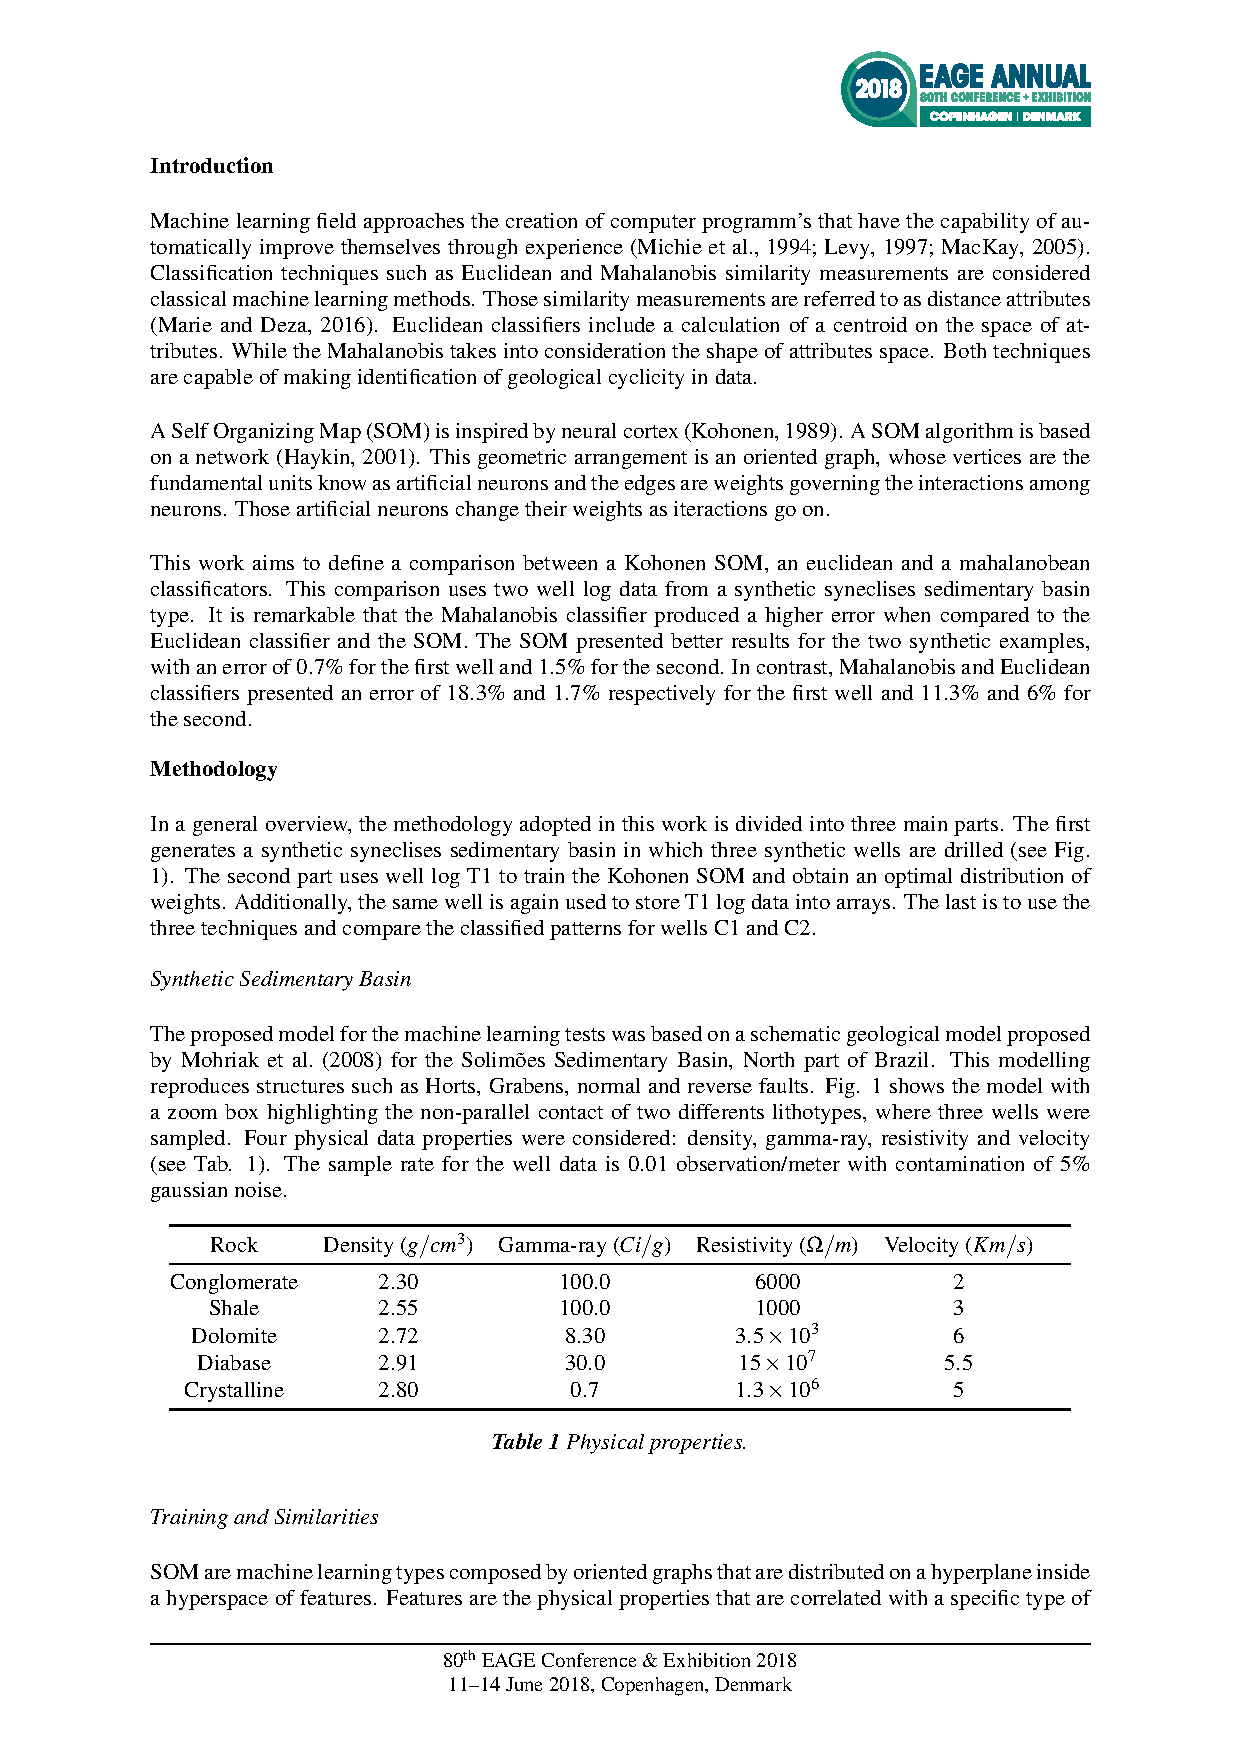
\includepdf[pages=1-4]{carreiraEAGE2018.pdf}
\end{document} 